\documentclass[11pt,a4paper]{report}

\usepackage[spanish, es-tabla]{babel}
\usepackage[utf8]{inputenc}
\usepackage{url}
\usepackage{url}

\usepackage{amsmath}
\usepackage{amsfonts}
\usepackage{amssymb}

\usepackage{graphicx}
\usepackage{float}
\usepackage{booktabs}

\usepackage{listings}
\usepackage{xcolor}
\definecolor{codegreen}{rgb}{0,0.6,0}
\definecolor{codegray}{rgb}{0.5,0.5,0.5}
\definecolor{codepurple}{rgb}{0.58,0,0.82}
\definecolor{backcolour}{rgb}{0.95,0.95,0.92}
\lstset{
    backgroundcolor=\color{backcolour},   
    commentstyle=\color{codegreen},
    keywordstyle=\color{magenta},
    numberstyle=\tiny\color{codegray},
    stringstyle=\color{codepurple},
    basicstyle=\ttfamily\footnotesize,
    breakatwhitespace=false,         
    breaklines=true,
    captionpos=b,
    keepspaces=true,                 
    numbers=left,
    numbersep=5pt,                  
    showspaces=false,                
    showstringspaces=false,
    showtabs=false,                  
    tabsize=2,
    language=Python
}

\usepackage{datetime}

\newdateformat{monthyeardate}{\monthname[\THEMONTH], \THEYEAR}

\begin{document}

\begin{titlepage}
    \centering
    
    {\textbf{Universidad de Guadalajara}}\\[0.5cm]
    {Centro Universitario de Guadalajara}\\[0.5cm]
    {Licenciatura en Inteligencia Artificial y Ciencia de los Datos}\\[2cm]
    
    {\textbf{Reporte técnico de resultados de JAPI para proyección de ventas diarias}}\\
    {Angel E. Moreno, Paulo A. Jiménez, Irving G. Robles y Juan P. Estrada}
    
    \vfill
    
    {Guadalajara, Jalisco \par}
    \monthyeardate\today
    
\end{titlepage}

\tableofcontents
\newpage

\section{Introducción}
El entorno competitivo actual en el sector comercial exige que las organizaciones adopten enfoques analíticos avanzados
para optimizar la toma de decisiones estratégicas, particularmente en la gestión de inventarios y la planificación financiera.

En este contexto se sitúa Urvet de México, una organización dedicada a la distribución mayorista de productos farmacéuticos,
biológicos, alimenticios y accesorios especializados para el sector veterinario y de la salud animal.
Su operación comercial abarca una compleja red de suministro que atiende a clínicas, hospitales veterinarios y centros de distribución minoristas.
Esta dinámica comercial genera un flujo constante de datos transaccionales con un alto potencial de explotación para el desarrollo de ventajas competitivas.
Al enfrentarse a un mercado con demandas altamente variables, influenciadas por factores estacionales que afectan
la prevalencia de ciertas condiciones de salud animal, o campañas de abastecimiento clínico, la predictibilidad de sus ingresos se convierte en un pilar operativo crítico.

Con el propósito de transformar este activo analítico en valor predictivo, se ha diseñado el Proyecto JAPI, denominado así a partir de las iniciales
de los integrantes del equipo de trabajo. Este proyecto surge como un esfuerzo integrador de ciencia de datos aplicado a la infraestructura operativa de Urvet,
utilizando sus registros históricos de transacciones comerciales como la fuente primaria de información.

El núcleo técnico de la investigación se centra en la incorporación, entrenamiento y evaluación comparativa de tres arquitecturas
de modelado de series de tiempo de distinta naturaleza: el modelo estadístico lineal SARIMAX, el modelo aditivo basado en curvas de crecimiento Prophet,
y la red neuronal recurrente LSTM (Long Short-Term Memory).

La variable objetivo fundamental para este análisis es la proyección de las ventas netas, definida estrictamente como las ventas totales de la
organización tras deducir los descuentos comerciales y las devoluciones de producto, calculadas antes de la aplicación de cargas impositivas.
Si bien el horizonte de planeación y visualización estratégica se proyectará de manera mensual, el pipeline de datos está diseñado para procesar
la información y generar los pronósticos con una granularidad diaria. Este nivel de detalle analítico permitirá capturar patrones de estacionalidad intra-semanal,
días festivos y efectos de calendario que suelen diluirse en agregaciones macro, sentando las bases para un análisis profundo de la morfología y comportamiento
de los datos que se desglosará en las secciones subsecuentes de este documento.

\section{Objetivos}

\subsection{Objetivo General}
Desarrollar e implementar un sistema predictivo robusto para la proyección de ventas netas mensuales con granularidad diaria utilizando
los datos históricos de la empresa Urvet, mediante la evaluación comparativa de los modelos SARIMAX, Prophet y LSTM, con el fin de
determinar la arquitectura con mayor precisión y capacidad de generalización.

\subsection{Objetivos Específicos}
\begin{itemize}
    \item Extracción y Modelado.
    Diseñar e implementar un pipeline eficiente para la extracción, 
    limpieza y agregación de los datos transaccionales de Urvet, garantizando el cálculo preciso de las ventas netas diarias antes de impuestos.

    \item Tratamiento Estadístico.
    Desarrollar mecanismos automatizados para la identificación y el tratamiento de valores atípicos \textit{outliers}
    y anomalías en las series de tiempo mediante múltiples estrategias de imputación.

    \item Evaluación Comparativa.
    Evaluar el rendimiento de un modelo estadístico clásico \textit{SARIMAx}, un enfoque de descomposición estructural \textit{Prophet}
    y un modelo de aprendizaje profundo \textit{LSTM} utilizando métricas de error estandarizadas.

    \item Optimización Computacional.
    Analizar la complejidad algorítmica y el costo computacional de cada arquitectura
    para asegurar la viabilidad y escalabilidad del sistema en un entorno de producción.

\end{itemize}

\section{Metodología}
El desarrollo del Proyecto JAPI se fundamentó en un enfoque metodológico de arquitectura modularizada,
diseñado bajo principios de alta cohesión y bajo acoplamiento.

Esta estructura no solo garantiza la escalabilidad del sistema predictivo, sino que aisla rigurosamente
cada etapa del ciclo de vida del dato, mitigando el riesgo de fuga de información y optimizando
la reproducibilidad de los experimentos. El flujo de trabajo se articuló mediante un pipeline secuencial
y robusto que transiciona orgánicamente desde la ingesta de las fuentes transaccionales crudas de Urvet de México
hasta el despliegue del motor de evaluación comparativa de los modelos.

La arquitectura del sistema se encuentra segmentada en tres grandes módulos interdependientes:
\begin{itemize}
    \item Adquisición e Ingesta de Datos.
    Capa encargada de la conexión, extracción y modelado de las bases de datos transaccionales.
    Este módulo centraliza las reglas de negocio para la consolidación de la variable objetivo,
    automatizando la extracción de la base de datos central de la empresa, cuidando la integridad de la misma.

    \item Procesamiento y Tratamiento Estadístico.
    Bloque especializado en el análisis exploratorio y la sanitización de las series temporales.
    A través de componentes orientados a objetos, este módulo computa dinámicamente máscaras lógicas
    vectorizadas para la detección de anomalías y desacopla la lógica de imputación,
    permitiendo al sistema despachar múltiples estrategias de corrección (como interpolaciones lineales o medias móviles vecinas)
    según la morfología del dato.

    \item Modelado Predictivo y Evaluación.
    Motor analítico donde convergen las arquitecturas SARIMAX, Prophet y LSTM.
    Este módulo administra de manera agnóstica el entrenamiento de los algoritmos y expone
    una interfaz estandarizada para someter los pronósticos a un marco riguroso de validación cruzada
    y métricas de error estadístico, garantizando una comparación simétrica del rendimiento predictivo.
\end{itemize}

    \subsection{Arquitectura del Repositorio y Estructura del Proyecto}
    Para dar soporte al enfoque modular propuesto, el sistema se organizó bajo una estructura de directorios
    estandarizada que separa las responsabilidades de configuración, experimentación, almacenamiento de artefactos y
    lógica productiva. A continuación se describe el propósito y contenido de cada componente del repositorio:

    \subsubsection{Capa de configuración y ejecución principal}
    \begin{itemize}
        \item \textit{config/}
        \item \textit{core/}
    \end{itemize}
    El directorio de configuración centraliza los parámetros estáticos y las credenciales operativas del sistema,
    evitando la persistencia de variables rígidas dentro del código fuente. Este espacio gestiona las cadenas de
    conexión a los servidores de bases de datos y define las variables de entorno necesarias para el despliegue del proyecto.
    Por otro lado, la sección del núcleo operativo funge como el centro de control de la ejecución,
    alojando las rutinas principales que importan los módulos reutilizables y coordinan secuencialmente las fases del pipeline completo.

    \subsubsection{Capa de datos y artefactos de modelado}
    El almacenamiento de información y persistencia de conocimiento se divide en dos repositorios específicos:
    \begin{itemize}
        \item \textit{data/}\\
        Este espacio está destinado al almacenamiento de las fuentes transaccionales en
        formatos crudos tales como archivos de valores separados por comas o hojas de cálculo electrónicas,
        sirviendo además como repositorio para los conjuntos de datos que ya han sido sometidos a
        los procesos de limpieza y normalización.

        \item \textit{models/}\\
        Funciona como un repositorio cerrado para la preservación de los
        modelos finales entrenados y las definiciones estructurales de datos,
        resguardando archivos de extensión h5 para la red neuronal recurrente,
        serializaciones numéricas para el modelo estadístico lineal o formatos de intercambio de datos tipo
        json para configuraciones específicas de los algoritmos.
    \end{itemize}

    \subsubsection{Entorno de experimentación y desarrollo}
    La fase de investigación y descubrimiento de insights se aisla por completo de la producción mediante un
    espacio exclusivo para libretas interactivas \textit{notebooks/}.
    Este directorio contiene únicamente archivos de extensión ipynb o reportes exportados en lenguaje de marcado
    de hipertexto que documentan los análisis visuales de tendencias, correlaciones y detección de anomalías.
    Bajo ninguna circunstancia este módulo provee lógica al flujo productivo del sistema.

    \subsubsection{Capa de lógica reutilizable y utilidades}
    El motor del proyecto reside en la sección de código fuente denominada \textit{src/},
    la cual se subdivide en componentes especializados que encapsulan la lógica interna del sistema:

    \begin{itemize}
        \item  \textit{db\_conn.py}\\
        Archivo que implementa de forma exclusiva la clase encargada de gestionar el ciclo de vida de
        la conexión y las consultas hacia la base de datos de la organización.

        \item  \textit{cleaner.py}\\
        Componente que agrupa las funciones de transformación y el despacho de algoritmos
        de corrección estadística una vez validada su funcionalidad operativa.

        \item  \textit{models.py}\\
        Módulo orientado a objetos cuyas clases administran de manera unificada los procesos de reentrenamiento,
        optimización de hiperparámetros, evaluación simétrica y generación de predicciones.
    \end{itemize}

    \subsection{Capa de resultados}

    Para mantener la lógica detrás de la estructura modularizada, se implementó un directorio exclusivo para el resguarde de datos predichos.

    \begin{itemize}
        \item \textit{forecast/}\\
        El tipo de datos almacenados continua con la accesibilidad a través de archivos de formato valores separados por comas, con el
        objetivo de que sean almacenados de forma fácil y ligera.
    \end{itemize}

    Finalmente, el módulo de utilidades  \textit{utils/utils.py} centraliza funciones de carácter universal que, por su naturaleza transversal,
    no pertenecen a una clase de negocio específica, proveyendo herramientas genéricas para la lectura de sistemas de archivos, la asignación
    estricta de tipos de datos o el formateo de marcas de tiempo.

    \subsection{Adquisición y Modelado de Datos}

        \subsubsection{Conexión a base de datos}
        La estrategia de seguridad y desacoplamiento de la infraestructura analítica se fundamenta en el aislamiento de las variables
        críticas del sistema. Para evitar la exposición de credenciales dentro del código fuente, se implementó un esquema basado en archivos
        externos de entorno, los cuales resguardan los parámetros de autenticación tanto del servidor de bases de datos como del nodo intermedio
        de comunicación segura.

        El script de configuración inicial lee dinámicamente estas variables operativas y utiliza herramientas de resolución de rutas del sistema
        operativo para establecer los caminos absolutos de los directorios del proyecto, garantizando la portabilidad del sistema en cualquier entorno
        de ejecución local. El código correspondiente a la inicialización de los entornos y asignación estática se detalla a continuación:

        \textit{config/settings.py}

        \begin{lstlisting}[language=Python, caption=Configuración de entornos y rutas globales en settings.py.]
import pathlib
import os
from dotenv import load_dotenv

load_dotenv()

DB_HOST = os.getenv('DB_HOST')
DB_PASSWORD = os.getenv('DB_PASSWORD')
DB_NAME = os.getenv('DB_NAME')
DB_PORT = os.getenv('DB_PORT')
DB_USER = os.getenv('DB_USER')

SSH_IP = os.getenv('SSH_IP')
SSH_PRIVATE_KEY = os.getenv('SSH_PRIVATE_KEY')
SSH_USERNAME = os.getenv('SSH_USERNAME')
SSH_PORT = os.getenv('SSH_PORT')

BASE_DIR = pathlib.Path(__file__).resolve().parent.parent

DATA_DIR = BASE_DIR / "data"
CONFIG_DIR = BASE_DIR / "config"
MODELS_DIR = BASE_DIR / "models"
SRC_DIR = BASE_DIR / "src"
NB_DIR = BASE_DIR / "notebooks"
FORECAST_DIR = BASE_DIR / "forecast"
        \end{lstlisting}

    \subsubsection{Extracción y consumo}
    Para interactuar de forma segura con los registros transaccionales de Urvet de México,
    se desarrolló una \textit{clase} que gestiona la comunicación mediante un túnel cifrado de shell segura.
    Esta técnica redirige el tráfico de la base de datos relacional a través de un puerto local virtualizado,
    evadiendo la necesidad de exponer los puertos del servidor hacia redes públicas.

    La clase implementada encapsula el ciclo de vida del canal de comunicación de forma automatizada.
    El método de conexión emplea bloques de control de excepciones y gestores de contexto para asegurar que los cursores y
    las conexiones con el motor de base de datos PostgreSQL se cierren correctamente tras la ejecución, mitigando la fuga de
    memoria o saturación de hilos en el servidor.
    
    Asimismo, la persistencia local se optimiza volcando las consultas directamente
    hacia estructuras de datos tabulares, facilitando la creación de archivos planos codificados en formato universal.
    La abstracción completa de esta lógica de conectividad se expone en el siguiente bloque de código:

    \textit{src/db\_conn.py}

    \begin{lstlisting}[language=Python, caption=Clase de gestión de conexión segura y persistencia en db\_conn.py.]
import psycopg2
import pandas as pd
from sshtunnel import SSHTunnelForwarder
from config.settings import (
    DB_HOST, DB_PASSWORD, DB_NAME, DB_PORT, DB_USER,
    SSH_IP, SSH_PRIVATE_KEY, SSH_USERNAME, SSH_PORT
)

class DatabaseConnection:
    def __init__(self, *, DB_HOST, DB_PASSWORD, DB_NAME, DB_PORT, DB_USER, SSH_IP, SSH_PRIVATE_KEY, SSH_USERNAME, SSH_PORT):
        self.db_host = DB_HOST
        self.db_password = DB_PASSWORD
        self.db_name = DB_NAME
        self.db_port = int(DB_PORT)
        self.db_user = DB_USER
        self.ssh_ip = SSH_IP
        self.ssh_username = SSH_USERNAME
        self.ssh_private_key = SSH_PRIVATE_KEY
        self.ssh_port = int(SSH_PORT)

    def setup_status(self):
        print(f'DB Host: {self.db_host} -> as {type(self.db_host)}')
        print(f'DB name: {self.db_name} -> as {type(self.db_name)}')
        if not self.db_password:
            raise ValueError('Password was not set correctly')
        else:
            print('Password: *')
        print(f'DB port: {self.db_port} -> as {type(self.db_port)}')
        print(f'DB username: {self.db_user} -> as {type(self.db_user)}')

    def set_connection(self, *, query: str = None):
        try:
            with SSHTunnelForwarder(
                (self.ssh_ip, int(self.ssh_port)),
                ssh_private_key=self.ssh_private_key,
                ssh_username=self.ssh_username,
                remote_bind_address=(self.db_host, int(self.db_port)),
                local_bind_address=('127.0.0.1', self.db_port),
                host_pkey_directories=[]
            ) as server:
                print('Server connected')
                params = {
                    'database': self.db_name,
                    'user': self.db_user,
                    'password': self.db_password,
                    'host': '127.0.0.1',
                    'port': server.local_bind_port
                }
                conn = psycopg2.connect(params)
                curs = conn.cursor()

                if query is None:
                    print("database connected")
                    curs.close()
                    conn.close()
                    return True
                else:
                    print(f'Query: {query}')
                    curs.execute(query)
                    headers = [desc[0] for desc in curs.description]
                    res = curs.fetchall()
                    curs.close()
                    conn.close()
                    return res, headers
        except Exception as e:
            print(f'Connection error. {e}')

    def query_to_csv(self, *, query: str = None, output_file_name: str = 'output.csv'):
        try:
            if not query:
                print("There is no query provided")
                return False
            data, headers = self.set_connection(query=query)
            df = pd.DataFrame(data, columns=headers)
            print("\nPreview\n")
            print(df.head())
            df.to_csv(output_file_name, index=False, encoding='utf-8')
            print(f"\nDF successfully created and saved as '{output_file_name}'")
            return df
        except Exception as e:
            print(f"Error while exporting to CSV: {e}")
            return False
    \end{lstlisting}

    \subsubsection{Modelado de datos}
    El proceso de modelado requiere una fase previa de estructuración y homogeneización de los tipos de datos transaccionales,
    garantizando que las series de tiempo posean la alineación matemática adecuada antes de ser inyectadas en las fases de entrenamiento analítico.

        \paragraph{Primer acercamiento.}
        El flujo de trabajo se inicializa en el componente ejecutor principal del sistema \textit{main.py}.
        En esta aproximación temprana, el pipeline realiza la instanciación del objeto de conexión, ejecuta una consulta masiva
        para recuperar la totalidad del histórico transaccional de ventas y genera el archivo plano intermedio en la ruta de
        almacenamiento de datos previamente resuelta. 

        Posteriormente, se lleva a cabo un proceso de alineación en los metadatos de la estructura relacional, forzando la
        conversión del identificador de ruta hacia un formato entero extendido con soporte para valores nulos y transformándolo
        finalmente en una cadena de texto homogénea.
        
        Esta transformación previene inconsistencias de indexación durante los cruces matriciales subsecuentes. El flujo operativo inicial se detalla a continuación:

        \textit{core/main.py}

        \begin{lstlisting}[language=Python, caption=Orquestación inicial e ingesta transaccional en main.py.]
from src.db_conn import DatabaseConnection
from src.models import SarimaxModel
from src.cleaner import Cleaner
from config.settings import (
    DB_HOST, DB_PASSWORD, DB_NAME, DB_PORT, DB_USER,
    SSH_IP, SSH_PRIVATE_KEY, SSH_USERNAME, SSH_PORT,
    DATA_DIR, FORECAST_DIR, MODELS_DIR
)
import pandas as pd
import json

def main():
    db_conn = DatabaseConnection(
        DB_HOST=DB_HOST, DB_NAME=DB_NAME, DB_PASSWORD=DB_PASSWORD,
        DB_PORT=DB_PORT, DB_USER=DB_USER, SSH_PRIVATE_KEY=SSH_PRIVATE_KEY,
        SSH_IP=SSH_IP, SSH_USERNAME=SSH_USERNAME, SSH_PORT=SSH_PORT
    )

    sales_query = """
    SELECT * FROM sale_transactions
    """
    output_path = f'{DATA_DIR}/sales.csv'

    sales = db_conn.query_to_csv(query=sales_query, output_file_name=output_path)
    sales['route_id'] = sales['route_id'].astype('Int64').astype(str)

if __name__ == '__main__':
    main()
        \end{lstlisting}


    \subsection{Análisis Exploratorio de Datos}
    El análisis exploratorio de datos constituye la fase analítica preliminar orientada a caracterizar la morfología de la información extraída,
    identificar anomalías estructurales y validar las propiedades estadísticas de las series de tiempo antes de su procesamiento predictivo.

        \subsubsection{Aislamiento del Entorno de Ejecución y Extracción Core}
        Para garantizar la reproducibilidad de las pruebas estadísticas y aislar el entorno de desarrollo interactivo del pipeline de producción,
        se implementó una rutina de resolución dinámica de rutas del sistema que inyecta el directorio raíz en el camino de búsqueda de los módulos del sistema.
        Esto permite reutilizar los componentes de conectividad previamente desarrollados.
        
        El bloque de inicialización de librerías científicas y configuración de formatos numéricos se presenta a continuación:

        \textit{notebooks/eda.ipynb}

        \begin{lstlisting}[language=Python, caption=Configuración del entorno interactivo e importación de dependencias.]
from pathlib import Path
import sys

ROOT_DIR = Path.cwd().parent

if str(ROOT_DIR) not in sys.path:
    sys.path.insert(0, str(ROOT_DIR))

from src.db_conn import DatabaseConnection
from config.settings import (
    DB_HOST, DB_PASSWORD, DB_NAME, DB_PORT, DB_USER,
    SSH_IP, SSH_PRIVATE_KEY, SSH_USERNAME, SSH_PORT, DATA_DIR
)

import pandas as pd
pd.options.display.float_format = '{:,.2f}'.format

import numpy as np
import matplotlib.pyplot as plt
import seaborn as sns

from statsmodels.tsa.seasonal import seasonal_decompose
from statsmodels.tsa.stattools import adfuller
        \end{lstlisting}

        Tras mapear el catálogo global de la base de datos operativa de Urvet de México, se identificaron cuarenta y nueve entidades relacionales activas.
        Con el objetivo de optimizar los recursos de cómputo y focalizar el esfuerzo analítico en el comportamiento transaccional del mercado,
        el alcance de la investigación se delimitó estrictamente a la extracción de dos entidades núcleo:
        la tabla maestro de clientes y el registro histórico de transacciones de venta.

        La persistencia de estas entidades en archivos planos asegura que cada corrida del pipeline cuente con una evidencia inmutable
        del último conjunto de datos utilizado, facilitando las auditorías del modelo. El proceso de extracción interactivo se detalla en el siguiente segmento de código:

        \textit{notebooks/eda.ipynb}

        \begin{lstlisting}[language=Python, caption=Consumo y persistencia local de las entidades relacionales core.]
new_conn = DatabaseConnection(
    DB_HOST=DB_HOST, DB_NAME=DB_NAME, DB_PASSWORD=DB_PASSWORD,
    DB_PORT=DB_PORT, DB_USER=DB_USER, SSH_PRIVATE_KEY=SSH_PRIVATE_KEY,
    SSH_IP=SSH_IP, SSH_USERNAME=SSH_USERNAME, SSH_PORT=SSH_PORT
)

sale_transactions_query = """
SELECT * FROM sale_transactions
"""

customers_query = """
SELECT * FROM customers
"""

new_conn.setup_status()
new_conn.query_to_csv(query=sale_transactions_query, output_file_name=DATA_DIR / 'sales.csv')
new_conn.query_to_csv(query=customers_query, output_file_name=DATA_DIR / 'customers.csv')
        \end{lstlisting}

        \subsubsection{Carga de Datos e Inspección de Estructuras}
        Una vez realizado el volcado de la base de datos, las fuentes se cargan en estructuras tabulares en memoria para validar su correcta disposición columnar.
        La tabla maestro de clientes provee los atributos críticos para la futura segmentación comercial, incluyendo identificadores, fechas de alta operativas y límites de crédito.
        Por su parte, la tabla de transacciones de venta constituye el núcleo temporal del proyecto, registrando las marcas de tiempo,
        los costos totales y los precios netos requeridos por los modelos de aprendizaje profundo y econométricos.

            \begin{lstlisting}[language=Python, caption=Lectura de los conjuntos de datos hacia estructuras tabulares.]
customers = pd.read_csv(DATA_DIR / 'customers.csv')
sales = pd.read_csv(DATA_DIR / 'sales.csv')

display(customers.head())
display(sales.head())
            \end{lstlisting}

        \subsubsection{Evaluación de Completitud e Integridad del Corpus}
        La calidad del modelado de series de tiempo depende críticamente de la continuidad de los registros.
        Por ello, se ejecutó una rutina de auditoría de valores faltantes sobre cada matriz con la finalidad de trazar un mapa de nulidades.
        El diagnóstico del estado de completitud se procesó mediante el siguiente script:

            \begin{lstlisting}[language=Python, caption=Auditoría de valores nulos en los conjuntos de datos.]
print('Conteo de nulos de sales')
print(sales.isna().sum())

print('Conteo de nulos de customers\n')
print(customers.isna().sum())
            \end{lstlisting}

        Los resultados demuestran que la estructura de clientes presenta una integridad absoluta con cero registros nulos en todas sus dimensiones.
        En contraparte, la matriz transaccional exhibe seiscientas ochenta y nueve ausencias en el identificador de producto y tres mil setenta
        y ocho nulidades en el identificador de ruta comercial. 

        Desde una perspectiva de negocio, estas anomalías indican transacciones globales no vinculadas a canales de distribución específicos o
        registros huérfanos que demandarán una estrategia de filtrado o imputación guiada en las etapas subsecuentes, previniendo la distorsión
        de las tendencias por falta de consistencia geográfica.

    \subsection{Limpieza y Normalización}
    La fase de preprocesamiento técnico tiene como objetivo estandarizar las estructuras de los conjuntos de datos, asegurando la consistencia operativa antes de la agregación temporal.
    Este proceso es un requisito crítico debido a que el sistema operará bajo diferentes niveles de granularidad para satisfacer las demandas de proyecciones
    macro es decir, análisis globales diarios o segmentados por centro de distribución y proyecciones micro,
    las cuales requieren un nivel de detalle diario por ruta comercial o consolidaciones mensuales por cliente. 

    Dado que el análisis se ejecuta estrictamente sobre las ventas netas, la presencia de notas de crédito y registros atípicos requiere un proceso riguroso de tipado y
    sanitización para asegurar que las transformaciones posteriores permitan a los modelos clásicos y de aprendizaje profundo discriminar
    correctamente las señales de la demanda.

    \subsubsection{Estandarización de Formatos y Tipos de Datos}
    El primer paso operativo consistió en homologar los tipos de datos en la matriz transaccional, la cual cuenta con un histórico de seiscientos noventa
    y siete mil setecientos cincuenta registros.
    Se transformó la variable temporal mediante un proceso de conversión explícita hacia estructuras cronológicas de alta precisión,
    anulando cualquier registro que presente inconsistencias de origen. 

    De forma paralela, las columnas financieras y de conteo de existencias se castearon hacia valores numéricos de punto flotante de sesenta y cuatro bits,
    mientras que los identificadores categóricos se unificaron en cadenas de texto homogéneas, implementando un tratamiento especial para el identificador
    de rutas comerciales mediante un tipo entero extendido. El snippet para este proceso se detalla a continuación:

    \textit{notebooks/eda.ipynb}

        \begin{lstlisting}[language=Python, caption=Homologación de tipos de datos macro y micro en la matriz de ventas.]
sales['sale_date'] = pd.to_datetime(sales['sale_date'], errors='coerce')

num_cols = [
    'total_cost', 'net_price', 'gross_price', 'profit', 'quantity'
]

cat_cols = [
    'customer_id', 'product_id', 'product_class_id', 'warehouse_id', 'route_id'
]

for col in num_cols:
    sales[col] = pd.to_numeric(sales[col], errors='coerce').astype(float)

for col in cat_cols:
    if col == 'route_id':
        sales[col] = sales[col].astype('Int64').astype(str)
    else:
        sales[col] = sales[col].astype(str)
        \end{lstlisting}

    \subsubsection{Imputación de Valores Nulos}
    Para evitar la pérdida de registros históricos y mantener la integridad total de las observaciones transaccionales,
    se rechazó la estrategia de eliminación física de filas. En su lugar, se optó por un enfoque de imputación por categorías genéricas
    explícitas para las variables de ruta y producto. 

    Este procedimiento sustituye las ausencias lógicas detectadas previamente por etiquetas de texto estructuradas, lo cual permite conservar
    la trazabilidad de la facturación global sin alterar la consistencia de las agrupaciones geográficas,
    logrando reducir el conteo de valores nulos a cero en todo el corpus operativo. La implementación de este proceso se detalla
    en el siguiente fragmento de código:

    \textit{notebooks/eda.ipynb}

        \begin{lstlisting}[language=Python, caption=Algoritmo de imputación categórica para variables de control.]
sales['route_id'] = sales['route_id'].fillna('ruta no especificada')
sales['product_id'] = sales['product_id'].fillna('producto no asignado')

print('Conteo de nulos de sales')
print(sales.isna().sum())
sales.info()
        \end{lstlisting}

    \subsubsection{Reconocimiento de Medidas de Tendencia Central y Análisis de Anomalías}
    Una vez removido el identificador subyacente y consolidada la estructura limpia del dataframe, se calcularon los
    estimadores estadísticos fundamentales sobre las variables numéricas de la matriz transaccional para auditar
    la distribución real de las operaciones financieras.

    Los resultados numéricos demuestran una asimetría severa hacia la derecha en la distribución de los ingresos de Urvet de México.
    El precio neto de las transacciones presenta una media de mil doscientos noventa y dos unidades monetarias con dieciocho centavos,
    mientras que el valor de la mediana se posiciona marcadamente por debajo, situándose en seiscientas veinticuatro unidades con veintinueve centavos.
    Esta brecha, sumada a una desviación estándar elevada de doce mil treinta y cuatro unidades con ochenta y cuatro centavos, confirma la dispersión
    natural del modelo de distribución mayorista, donde el comportamiento habitual está compuesto por órdenes veterinarias base de bajo valor,
    interrumpidas esporádicamente por picos de facturación masivos que alcanzan un valor máximo absoluto de dos millones quinientas cuarenta mil seiscientas
    noventa y siete unidades con treinta y seis centavos.

    El hallazgo más crítico de esta inspección estadística reside en los valores mínimos registrados en las dimensiones financieras.
    El precio neto y la utilidad mínima exhiben valores negativos extremos de menos cuatro millones doscientas treinta y tres mil seiscientas
    treinta y cuatro unidades con cincuenta y ocho centavos, un patrón que se correlaciona directamente con un volumen mínimo negativo de menos
    mil ochocientas cuarenta y cinco unidades de producto. 

    En la lógica de negocio de la organización, estos registros negativos representan la aplicación de notas de crédito comerciales,
    correcciones contables o devoluciones masivas de inventario. Debido a que las arquitecturas predictivas SARIMAX, Prophet y LSTM asumen distribuciones
    continuas y valores no invertidos para modelar la demanda regular, la presencia de estos valores negativos distorsiona el aprendizaje de las curvas de
    tendencia, marcando la necesidad imperativa de diseñar transformaciones y filtros específicos en la siguiente etapa del pipeline.


    \subsubsection{Visualización de Distribuciones}
    El análisis visual de las desviaciones estándar y los rangos de dispersión se consolidó mediante la generación de diagramas de caja y bigotes.
    Estos componentes gráficos permiten identificar de manera geométrica la concentración de los datos transaccionales, la localización de los rangos
    intermedios y la extensión de sus colas extremas.

        \paragraph{Exploración General del Corpus Transaccional.}
        Como primera aproximación, se sometió la variable de precio neto a una rutina de graficación para mapear la totalidad de los registros de venta,
        exponiendo la dispersión absoluta de la operación comercial de Urvet de México sin aplicar filtros geográficos o de canal.
        El snippet desarrollado se detalla a continuación:

        \textit{notebooks/eda.ipynb}

            \begin{lstlisting}[language=Python, caption=Construcción del diagrama de caja general para el precio neto.]
sns.set_theme(style="white")
plt.figure(figsize=(10, 4), dpi=100)

sns.boxplot(
    x=sales_prep['net_price'],
    color='#4361ee',
    width=0.4,
    linewidth=1.8,
    fliersize=4,
    flierprops={
        'markerfacecolor': '#e63946',
        'markeredgecolor': 'none',
        'alpha': 0.5
    }
)

plt.title('Distribucion general de venta neta', fontsize=14, pad=15, fontweight='bold', color='#212529')
plt.xlabel('Precio Neto ($)', fontsize=11, labelpad=10, color='#495057')

sns.despine(left=True)
plt.grid(axis='x', linestyle='--', alpha=0.5)

plt.tight_layout()
plt.show()
            \end{lstlisting}

            \begin{figure}[H]
                \centering
                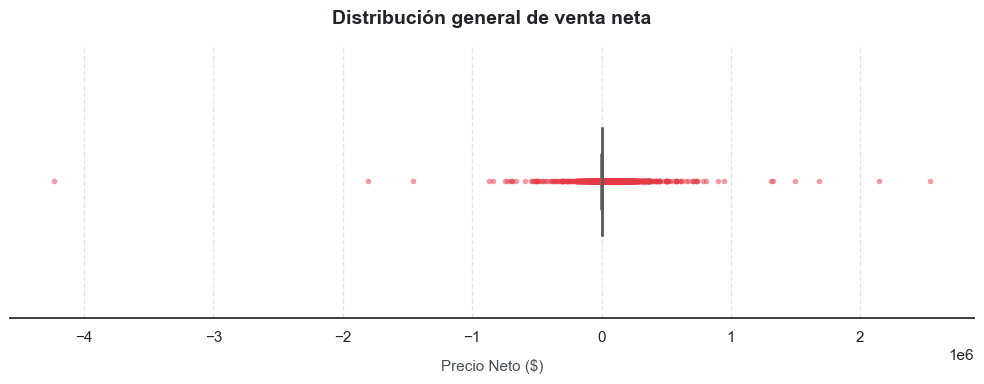
\includegraphics[width=0.9\textwidth]{img/distribucion_general_ventas.png}
                \caption{Distribución geométrica general de la variable precio neto transaccional.}
                \label{fig:dist_general}
            \end{figure}

        \paragraph{Aislamiento de la Operación Tradicional.}
        Al evaluar el primer diagrama, se detectó una distorsión masiva inducida por operaciones en los extremos de la distribución. Con el objetivo de aislar el comportamiento de los canales de venta físicos, se procedió a remover del conjunto de datos la ruta noventa, la cual corresponde exclusivamente al canal de comercio electrónico, debido a que su dinámica transaccional difiere del modelo de distribución mayorista tradicional. El proceso de filtrado y su correspondiente representación gráfica se detallan a continuación:

    \textit{notebooks/eda.ipynb}
    \begin{lstlisting}[language=Python, caption=Filtrado del canal de comercio electrónico y generación de la distribución corregida.]
    sales_wn_90 = sales_prep[sales_prep['route_id'] != '90']

    sns.set_theme(style="white")
    plt.figure(figsize=(10, 4), dpi=100)

    sns.boxplot(
        x=sales_wn_90['net_price'],
        color='#4361ee',
        width=0.4,
        linewidth=1.8,
        fliersize=4,
        flierprops={
            'markerfacecolor': '#e63946',
            'markeredgecolor': 'none',
            'alpha': 0.5
        }
    )

    plt.title('Distribucion general de venta neta sin ruta 90 ecommerce', fontsize=14, pad=15, fontweight='bold', color='#212529')
    plt.xlabel('Precio Neto ($)', fontsize=11, labelpad=10, color='#495057')

    sns.despine(left=True)
    plt.grid(axis='x', linestyle='--', alpha=0.5)

    plt.tight_layout()
    plt.show()
    \end{lstlisting}

    \begin{figure}[H]
        \centering
        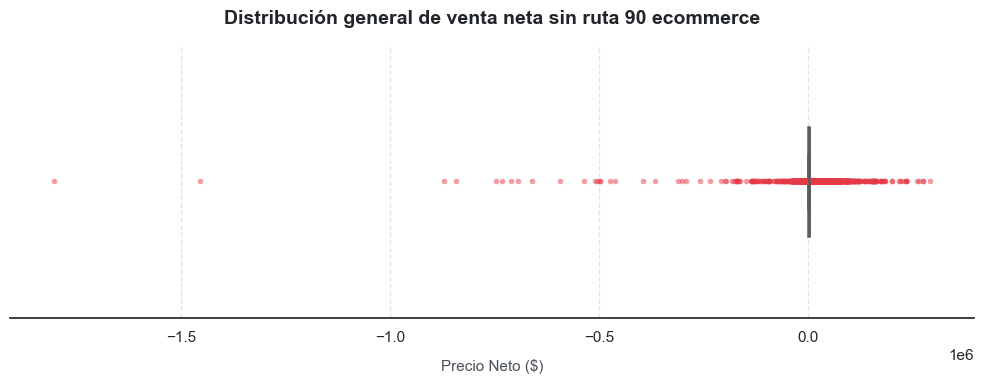
\includegraphics[width=0.9\textwidth]{img/distribucion_general_ventas_sin_r90.png}
        \caption{Distribución del precio neto tras la exclusión de las transacciones de comercio electrónico.}
        \label{fig:dist_sin_90}
    \end{figure}

        \paragraph{Segmentaci\'on por Centros de Distribuci\'on.}
        Para comprender la procedencia de las dispersiones extremas, se segment\'o la matriz filtrada por cada centro de
        distribuci\'on activo en la organizaci\'on. Este nivel de granularidad expone el comportamiento log\'istico individual y
        las diferencias operativas entre las regiones geogr\'aficas, implementando la siguiente rutina de visualizaci\'on:

    \textit{notebooks/eda.ipynb}
    \begin{lstlisting}[language=Python, caption=Comparativa de distribuciones financieras segmentada por almac\'en de origen.]
    sns.set_theme(style="white")
    plt.figure(figsize=(10, 6), dpi=100)

    sns.boxplot(
        data=sales_wn_90,
        x='net_price',
        y='warehouse_id',
        hue='warehouse_id',
        palette='Set2',
        width=0.5,
        linewidth=1.8,
        fliersize=4,
        flierprops={
            'markerfacecolor': '#e63946',
            'markeredgecolor': 'none',
            'alpha': 0.4
        }
    )

    plt.title('Comparativa de Venta Neta por CEDIS (Sin Ruta 90 E-commerce)', fontsize=14, pad=15, fontweight='bold', color='#212529')
    plt.xlabel('Precio Neto ($)', fontsize=11, labelpad=10, color='#495057')
    plt.ylabel('Centro de Distribuci\'on (CEDIS)', fontsize=11, labelpad=10, color='#495057')

    sns.despine(left=True, trim=True)
    plt.grid(axis='x', linestyle='--', alpha=0.5)

    plt.tight_layout()
    plt.show()
    \end{lstlisting}

    \begin{figure}[H]
        \centering
        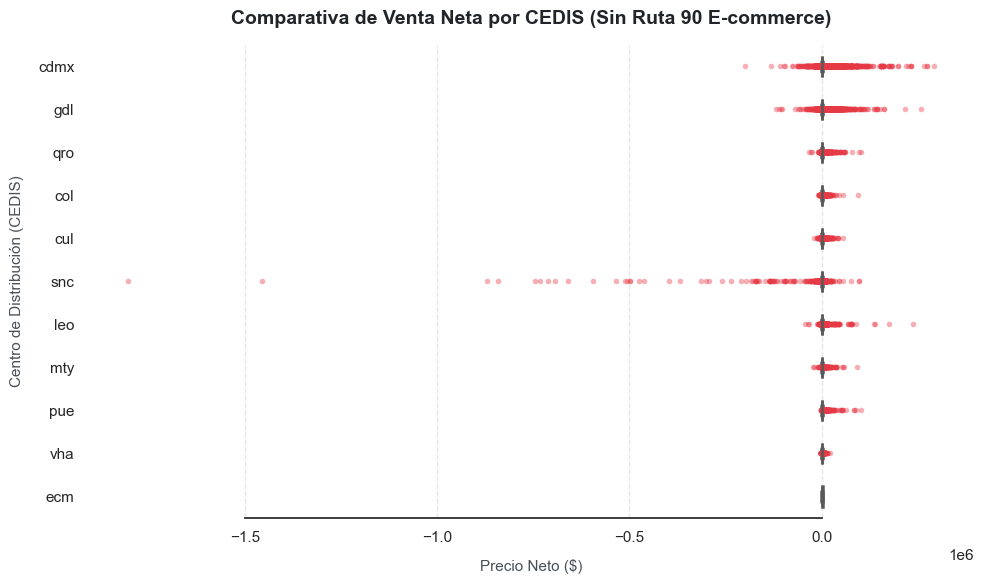
\includegraphics[width=0.9\textwidth]{img/comparativa_cedis.png}
        \caption{An\'alisis comparativo de dispersi\'on y valores at\'ipicos entre los diferentes centros de distribuci\'on.}
        \label{fig:comp_cedis}
    \end{figure}

        \paragraph{Criterio Estad\'istico contra la Naturaleza del Negocio.}
        Matem\'aticamente, la librer\'ia gr\'afica utilizada no eval\'ua los datos con base en el promedio,
        sino que emplea el rango intercuart\'ilico para delimitar los umbrales de normalidad estad\'istica.
        La caja central abarca el cincuenta por ciento de las transacciones comerciales, comprendido desde el primer cuartil
        hasta el tercer cuartil. Los l\'imites m\'aximo y m\'inimo permisibles para la declaraci\'on de valores ordinarios se
        encuentran modelados por las siguientes expresiones:

        $$ \text{L\'imite Superior} = Q_3 + 1.5 \times \text{IQR} $$
        $$ \text{L\'imite Inferior} = Q_1 - 1.5 \times \text{IQR} $$

        Cualquier registro transaccional que exceda estos umbrales calculados es representado en los diagramas como un punto
        rojo aislado identificado anal\'iticamente como un outlier o valor at\'ipico. 

        En el contexto operativo de Urvet de M\'exico, la inmensa mayor\'ia de los comprobantes generados
        en las rutas comerciales corresponden a compras cotidianas de bajo volumen, lo que provoca que la caja se comprima
        severamente cerca del origen num\'erico cero. Cuando ocurren eventos comerciales de alto impacto, la escala matem\'atica se rompe,
        dividi\'endose en dos fen\'omenos corporativos espec\'ificos:
        \begin{itemize}
            \item Picos positivos. Pedidos especiales ejecutados por distribuidores pesados que realizan compras de gran volumen por montos
            de cientos de miles o millones de pesos de forma espor\'adica.
            \item Picos negativos. Generaci\'on de notas de cr\'edito comerciales masivas y devoluciones de mercanc\'ia de gran escala que
            impactan directamente el indicador de precio neto de venta.
        \end{itemize}

        \paragraph{Evaluación Operativa por Centros de Distribución.}
        El análisis de los diagramas segmentados permite categorizar el comportamiento del mercado en tres perfiles de operación claros:
        \begin{itemize}
            \item Centro de distribución sin clasificar.\\
            Identificado con la etiqueta snc, presenta una dispersión atípica masiva en el espectro negativo, registrando movimientos que
            alcanzan valores de menos uno punto cinco millones de pesos. Este comportamiento dicta la existencia de devoluciones consolidadas
            o notas de crédito de gran escala aplicadas a cuentas corporativas. Sin embargo, este comportamiento es completamente normal considerando
            que este centro se emplea para registrar ajustes contables de rutas o clientes que ya no existen. Por lo tanto, no es viable eliminar
            estos registros, debido a que se siguen utilizando día con día y forman parte del comportamiento logístico e histórico de la organización.

            \item Centros de distribución de Guadalajara y Ciudad de México.\\
            Etiquetados como gdl y cdmx respectivamente, muestran las colas de puntos atípicos más largas en el espectro positivo. Estas
            regiones geográficas concentran a los clientes mayoristas con mayor poder de compra, rompiendo constantemente los techos de venta promedio de la ruta tradicional.

            \item Centro de distribución de comercio electrónico.\\Identificado como ecm, muestra una distribución compacta y libre de valores
            atípicos significativos, lo cual se logró gracias a la remoción previa de la ruta noventa del canal digital.
        \end{itemize}

        \subsubsection{Agrupaciones y Transformaciones de Frecuencia}
            La naturaleza transaccional de los registros crudos demanda una transformación estructural para posibilitar
            el modelado de series de tiempo. Para transicionar de un enfoque transaccional a uno temporal continuo,
            se aisló la columna de la fecha de venta, estableciéndola como el índice de la matriz de datos. Posteriormente,
            se ordenaron los registros de forma cronológica estricta para garantizar que las rutinas de remuestreo pudieran
            rellenar los vacíos temporales con ventas equivalentes a cero.
            
            Una vez indexado el conjunto, se aplicó una agrupación con frecuencia diaria sobre la variable de precio neto.
            Este procedimiento matemático consolida todos los ingresos registrados en una misma jornada, estructurando la serie
            continua de ochocientas sesenta y cinco observaciones que requieren los algoritmos predictivos.

        \begin{lstlisting}[language=Python, caption=Conversión de índice temporal y agrupación de ventas con frecuencia diaria.]
        sales_wn_90['sale_date'] = pd.to_datetime(sales_wn_90['sale_date'], errors='coerce')
        sales_date_index = sales_wn_90.set_index('sale_date')
        sales_date_index = sales_date_index.sort_index()

        sales_agg_daily = sales_date_index['net_price'].resample('D').sum()
        \end{lstlisting}

            \paragraph{Hallazgo de Anomalías Negativas Críticas.}
            A nivel transaccional, se habían detectado múltiples desviaciones severas. Al consolidar la serie de tiempo por día,
            el impacto de ciertas anomalías menores disminuyó gracias a la compensación natural con los ingresos positivos generados
            por las rutas. Sin embargo, la inspección gráfica de la evolución diaria de ingresos reveló un evento de extrema criticidad.

            Durante el mes de julio del año dos mil veinticuatro, la serie histórica registró una caída vertical atípica que arrastró
            el neto consolidado de toda la organización hasta menos dos punto cinco millones de pesos en una sola jornada. Al tratarse de
            un conjunto de datos agrupado por día, este hallazgo confirma que no se trata de un error de captura aislado, sino de un impacto
            financiero masivo, como la ejecución de una devolución corporativa o la aplicación de notas de crédito de gran escala, que distorsiona
            por completo la varianza normal del ecosistema comercial.

        \begin{figure}[H]
            \centering
            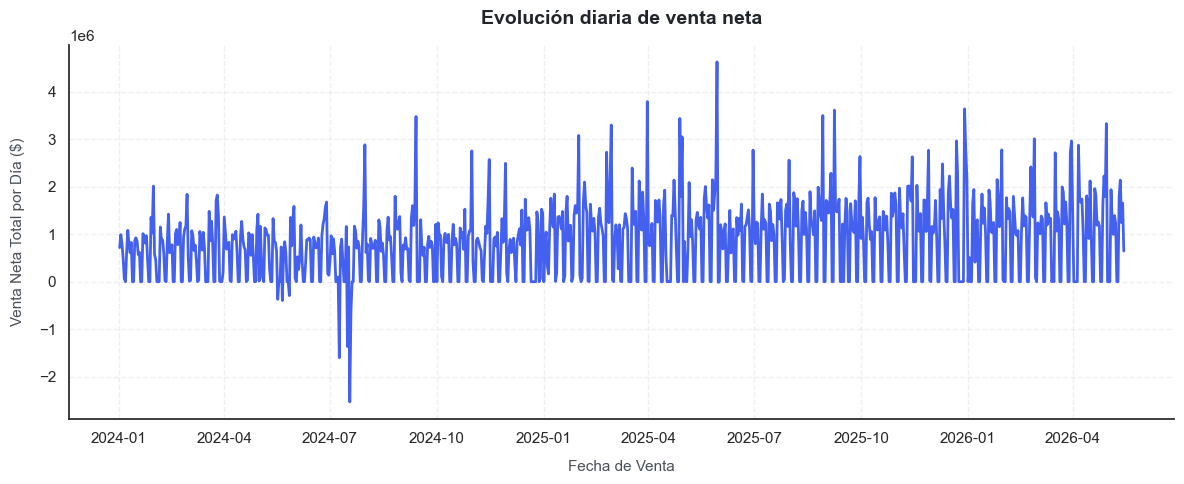
\includegraphics[width=0.9\textwidth]{img/evolucion_diaria_cruda.png}
            \caption{Evolución histórica diaria de la venta neta exponiendo la anomalía financiera.}
            \label{fig:evo_diaria_cruda}
        \end{figure}

            \paragraph{Identificación Visual de Estacionalidad Semanal.}
            De forma paralela a la detección de anomalías, la visualización de la evolución temporal expuso un comportamiento cíclico
            altamente repetitivo con una morfología de dientes de sierra. Se observan caídas sistemáticas que descienden de forma casi
            idéntica cada siete días, lapso que coincide de manera natural con los días de descanso o nula distribución en campo,
            seguidas inmediatamente por picos de surtido acelerado a mitad de semana. 
            
            Aunque este comportamiento cíclico será evaluado matemáticamente más adelante mediante funciones de autocorrelación,
            esta hipótesis visual robusta proporciona una guía estructural directa para la futura calibración de los hiperparámetros.
            En el caso del modelo SARIMAX, este comportamiento dicta la necesidad de configurar el parámetro de estacionalidad en siete periodos.

        \begin{figure}[H]
            \centering
            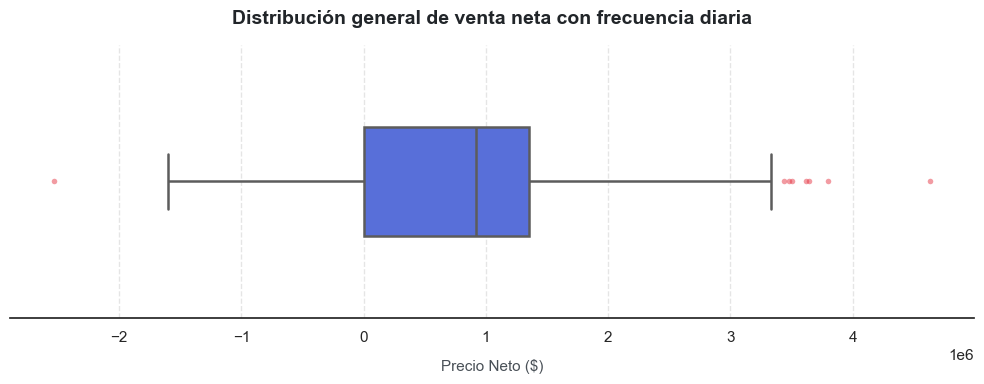
\includegraphics[width=0.9\textwidth]{img/boxplot_diario_crudo.png}
            \caption{Distribución agrupada diaria que expone los picos atípicos en ambos polos.}
            \label{fig:box_diario_crudo}
        \end{figure}

            \paragraph{Estrategias Opuestas para el Tratamiento de Valores Atípicos.}
            El análisis del diagrama de caja agrupado delimitó dos clases de puntos extremos que, dada su naturaleza de origen,
            requieren protocolos de limpieza diametralmente opuestos.
            
            Hacia el espectro positivo, el gráfico detectó siete registros que superaron masivamente el límite superior de normalidad,
            rompiendo techos de hasta cuatro punto seis millones de pesos diarios. A diferencia del evento de caída, estos picos
            revelan un patrón comercial sistemático e impulsado por el mercado: el efecto del cierre de mes y fin de trimestre.
            Las fechas de estos máximos históricos coinciden con las jornadas donde la fuerza de ventas de Urvet de México concentra
            operaciones de gran volumen para alcanzar cuotas de distribución. 
            
            Bajo este contexto, la directriz metodológica prohíbe estrictamente eliminar o suavizar los picos de facturación positiva,
            ya que representan la verdadera demanda límite de la cadena de suministro. Para que las arquitecturas predictivas capturen
            estos saltos dinámicos, el pipeline de datos implementará ingeniería de características mediante variables exógenas de intervención 
            temporal, permitiendo al algoritmo anticipar estos comportamientos.

            En contraparte, el polo negativo exige una corrección intrusiva. Preservar la caída de julio del dos mil veinticuatro sesgaría
            las predicciones futuras hacia abajo y deformaría los pesos de la red neuronal. Simultáneamente, eliminar la fila del registro
            destruiría la continuidad del calendario, provocando un error en cascada por la pérdida de la frecuencia temporal. Para solucionar
            esta inconsistencia matemática, se diseñó un protocolo de imputación por interpolación lineal.

        \begin{lstlisting}[language=Python, caption=Protocolo automatizado de interpolación lineal para limpieza de anomalías negativas.]
        sales_agg_daily_final = sales_agg_daily.copy()

        outs_days = sales_agg_daily_final[sales_agg_daily_final < 0].index
        print(f"Dias anomalos detectados por regla de negocio: {len(outs_days)}")

        sales_agg_daily_final[sales_agg_daily_final < 0] = np.nan
        sales_agg_daily_final = sales_agg_daily_final.interpolate(method='linear')
        \end{lstlisting}

            \paragraph{Consolidación de la Serie Limpia}
            El barrido automatizado identificó dieciocho días con balances netos negativos, una cifra que representa menos
            del dos por ciento del volumen de datos analizado. Ante esta proporción marginal, el algoritmo procedió a sustituir los
            montos de dichas jornadas por valores nulos, ejecutando inmediatamente una interpolación linear. Este método matemático
            calcula la pendiente entre el día previo y el posterior a la anomalía, uniendo ambos puntos mediante una recta que suaviza el
            cráter de forma local. Este mecanismo restaura la sanidad financiera de la serie de tiempo continua, conservando intacta la
            capacidad de la red para procesar la volatilidad operativa de los datos.

        \begin{figure}[H]
            \centering
            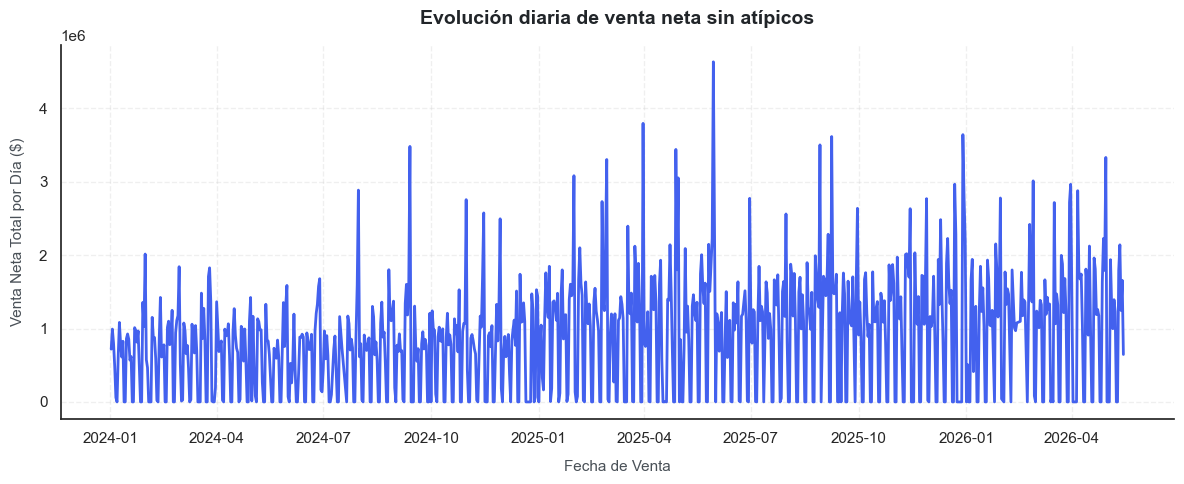
\includegraphics[width=0.9\textwidth]{img/evolucion_diaria_limpia.png}
            \caption{Serie de tiempo continua y estabilizada tras el proceso de interpolación matemática.}
            \label{fig:evo_diaria_limpia}
        \end{figure}

        \begin{figure}[H]
            \centering
            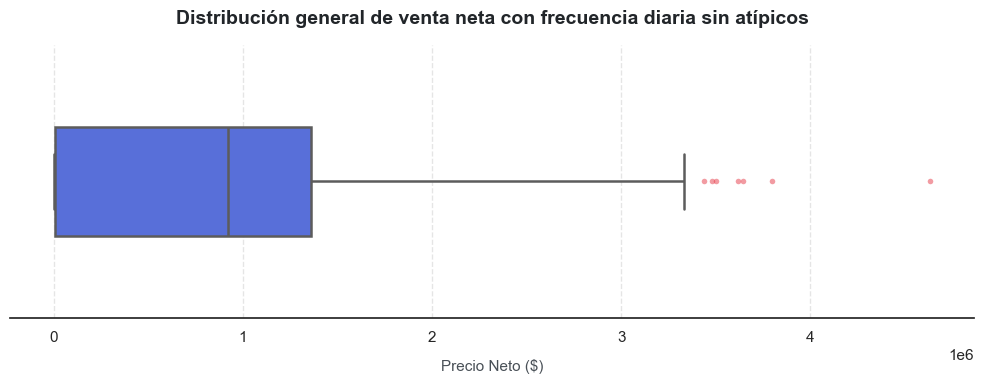
\includegraphics[width=0.9\textwidth]{img/boxplot_diario_limpio.png}
            \caption{Distribución final preservando exclusivamente los picos positivos operativos.}
            \label{fig:box_diario_limpio}
        \end{figure}

    \subsubsection{Pruebas de Hipótesis y Diagnóstico de Componentes}
        Antes de proceder a la fase de entrenamiento predictivo, resulta mandatorio desglosar los componentes
        estructurales subyacentes de la serie temporal mediante el planteamiento y ejecución de pruebas de hipótesis.
        Este diagnóstico permite validar si los datos cumplen con los supuestos matemáticos requeridos por los algoritmos
        estadísticos y define la necesidad de implementar transformaciones previas, tales como diferenciaciones o
        inclusión de variables exógenas.

        \paragraph{Estacionalidad y Descomposición Estructural.}
        Con el fin de confirmar numéricamente los patrones cíclicos observados durante la fase exploratoria,
        se aplicó un filtro de descomposición aditiva sobre la serie histórica diaria, aislando la tendencia general,
        la variabilidad estacional y el componente residual. 

        Considerando la hipótesis planteada en la visualización previa, se definió un periodo paramétrico de siete periodos.
        La instrumentación técnica de este proceso y su consecuente mapeo gráfico se exponen a continuación:

    \begin{lstlisting}[language=Python, caption=Descomposición aditiva y aislamiento del componente estacional.]
decompose = seasonal_decompose(sales_agg_daily_final, model='additive', period=7)

sns.set_theme(style="white")

observed = decompose.observed
trend = decompose.trend
seasonal = decompose.seasonal
resid = decompose.resid

fig, axes = plt.subplots(4, 1, figsize=(12, 10), sharex=True, dpi=100)

axes[0].plot(observed.index, observed.values, color='#4361ee', linewidth=1.5, alpha=0.8)
axes[0].set_ylabel('Venta Real ($)', fontsize=10, fontweight='bold', color='#495057')
axes[0].set_title('Descomposicion Analitica de la Serie Temporal (Ciclo Semanal, s=7)', 
                fontsize=14, pad=15, fontweight='bold', color='#212529')

axes[1].plot(trend.index, trend.values, color='#3f37c9', linewidth=2.2)
axes[1].set_ylabel('Tendencia ($)', fontsize=10, fontweight='bold', color='#495057')

axes[2].plot(seasonal.index, seasonal.values, color='#4cc9f0', linewidth=1.2)
axes[2].set_ylabel('Estacionalidad ($)', fontsize=10, fontweight='bold', color='#495057')

axes[3].scatter(resid.index, resid.values, color='#e63946', alpha=0.4, s=20)
axes[3].axhline(0, color='#212529', linestyle='-', linewidth=1, alpha=0.5)
axes[3].set_ylabel('Residuo ($)', fontsize=10, fontweight='bold', color='#495057')
axes[3].set_xlabel('Fecha de Venta', fontsize=11, labelpad=10, color='#495057')

for ax in axes:
    ax.grid(axis='both', linestyle='--', alpha=0.3)
    sns.despine(ax=ax, left=False, bottom=False)
    ax.tick_params(axis='both', labelsize=10, colors='#495057')

plt.tight_layout(h_pad=1.8)
plt.show()
    \end{lstlisting}

    \begin{figure}[H]
        \centering
        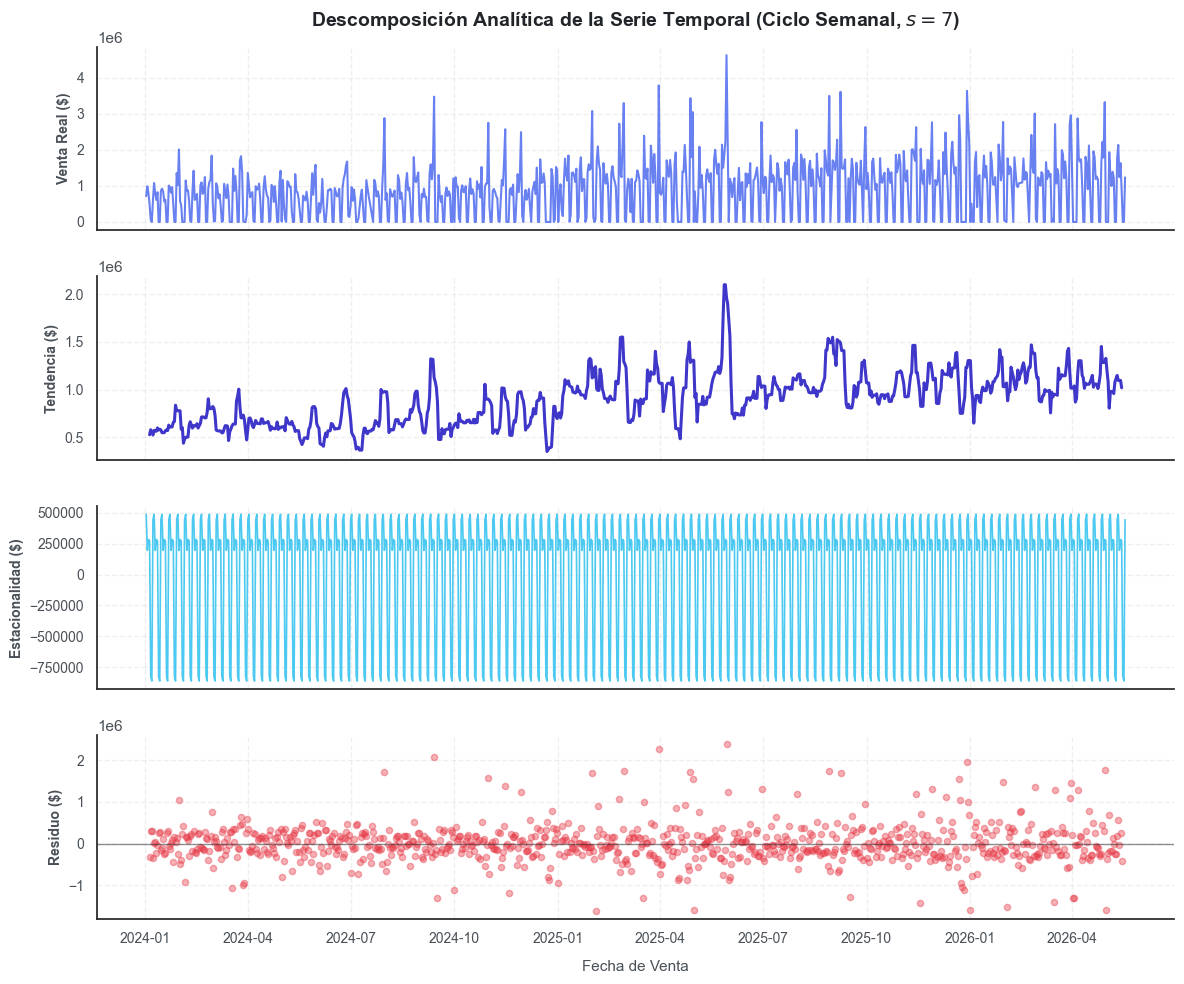
\includegraphics[width=0.9\textwidth]{img/descomposicion_serie.png}
        \caption{Aislamiento de la tendencia a largo plazo y comprobación visual del ciclo estacional de siete días.}
        \label{fig:descomposicion}
    \end{figure}

        Los hallazgos derivados de los paneles de descomposición proporcionan el sustento algorítmico para la configuración del pipeline:
        \begin{itemize}
            \item Consolidación de la estacionalidad.\\
            Existe evidencia gráfica contundente de un patrón estacional regular a lo largo de todo el histórico.
            El componente identifica un valle recurrente de menos setecientos cincuenta mil pesos respecto a la línea
            base durante los días de nula actividad logística, el cual es compensado de forma simétrica por crestas operativas.
            Este hallazgo rechaza la hipótesis nula de ausencia de temporalidad y bloquea de forma definitiva el hiperparámetro estacional
            de los modelos lineales en una frecuencia equivalente a un ciclo semanal continuo.

            \item Análisis del residuo comercial.\\
            El residuo representa la varianza que ni la tendencia de largo plazo ni el ciclo semanal lograron absorber.
            En condiciones ideales, este panel debería exhibir ruido blanco homogéneo. No obstante, se aprecian ráfagas de
            picos positivos que superan el millón de pesos de forma intermitente, coincidiendo exactamente con los días de cierre de mes.
            Esta evidencia justifica de manera obligatoria el diseño de una matriz exógena para inyectarla en la arquitectura SARIMAX,
            absorbiendo así el impacto de estos eventos comerciales sin corromper la memoria residual.
        \end{itemize}

        \paragraph{Prueba de Estacionariedad por Raíz Unitaria}
        Para garantizar que los estimadores predictivos no converjan hacia valores infinitos durante el cálculo de matrices de pesos,
        resulta fundamental validar si las propiedades estadísticas de la serie, específicamente su media y su varianza, permanecen constantes a lo largo del tiempo. 

        Con este fin, se ejecutó el test de Dickey-Fuller Aumentada bajo el siguiente marco de comprobación estadística:
        \begin{itemize}
            \item Hipótesis Nula.\\La serie de tiempo posee una raíz unitaria, implicando no estacionariedad, dependencia temporal fuerte y una media fluctuante.
            \item Hipótesis Alternativa.\\La serie carece de raíz unitaria, logrando estacionariedad y distribuyendo sus observaciones en torno a una media finita.
        \end{itemize}

    \begin{lstlisting}[language=Python, caption=Ejecución del test estadístico de Dickey-Fuller Aumentada.]
    result = adfuller(sales_agg_daily_final)

    print(f"ADF: {result[0]:.4f}")
    print(f"p-value: {result[1]:.4f}")
    print("Valores criticos:")
    for k, v in result[4].items():
        print(f"{k}: {v:.4f}")

    if result[1] <= 0.05:
        print("\n>> p-value <= 0.05, se rechaza H0, la serie es estacionaria")
    else:
        print("\n>> p-value > 0.05: no se rechaza H0. La serie no es estacionaria")
    \end{lstlisting}

        La ejecución arrojó un valor p de cero punto cero diecisiete, logrando superar el umbral estricto de significancia del cinco por ciento.
        Numéricamente, el estadístico de prueba dictaminó el rechazo de la hipótesis nula, catalogando la serie de ventas netas como estacionaria. 

        A pesar del veredicto matemático emitido por la prueba, el enfoque metodológico de un proyecto de ciencia de datos requiere un
        análisis holístico que trascienda la evaluación unidimensional.
        
        Al contrastar el estadístico de Dickey-Fuller contra el
        panel visual de la tendencia estructural aislado previamente en la Figura \ref{fig:descomposicion}, se identifica
        una discrepancia empírica severa. La línea de tendencia subyacente exhibe una pendiente ascendente prolongada a partir del
        segundo cuatrimestre del último año, indicando claramente que el crecimiento orgánico del negocio ha comenzado
        a alterar la media móvil histórica de la organización. 

        Por consiguiente, y como medida preventiva para maximizar la capacidad de ajuste algorítmico, las arquitecturas
        predictivas evaluarán configuraciones dinámicas que incluyan grados de diferenciación integral, el parámetro diferencial
        en los modelos ARIMA clásicos, con el objetivo de aplanar artificialmente cualquier rastro de inercia ascendente antes
        del entrenamiento computacional, blindando así los pronósticos contra un eventual sesgo exponencial.

            

\subsection{Ingeniería de Características}
El desarrollo y enriquecimiento de las variables de estudio se fundamenta en el conocimiento empírico derivado de la operación comercial logística de la organización. A partir de la experiencia directa del negocio, se identificaron factores temporales externos con alta probabilidad de influir en el volumen de demanda, los cuales resultan críticos para maximizar la capacidad de generalización y la precisión de las predicciones en etapas posteriores.

Entre las variables de mayor impacto aisladas para este estudio destacan tres eventos de calendario: en primer lugar, la validación de días feriados inactivos dictaminados por la legislación laboral; en segundo lugar, la identificación estricta de las jornadas de cierre de mes contable; y finalmente, el marcado de la zona de cierre operativo, la cual comprende los últimos tres días de cada ciclo mensual, periodo específico donde la fuerza de ventas concentra y acelera las transacciones de alto volumen.

Para instrumentar este conocimiento operativo en el entorno algorítmico, se procedió a transformar el índice temporal crudo en una matriz de características exógenas. Este arreglo matricial contiene indicadores lógicos binarios ceros y unos que actúan como banderas de intervención temporal. Posteriormente, esta matriz se concatenó de forma lateral con la serie de tiempo univariada, generando un conjunto de datos maestro preparado para ser consumido por las arquitecturas de aprendizaje profundo y estadístico. La implementación analítica se expone a continuación:

\begin{lstlisting}[language=Python, caption=Creación y concatenación de la matriz de características exógenas.]
exo_matrix = exo_matrix_mapping(sales_agg_daily_final)
master = pd.concat([sales_agg_daily_final, exo_matrix], axis=1)
\end{lstlisting}

La estructura resultante acopla la variable continua de precio neto con las tres dimensiones exógenas calculadas. Para ilustrar la consolidación de este conjunto maestro, se presenta el esquema de los registros finales donde se aprecian las activaciones de las banderas lógicas correspondientes a la zona de cierre y al fin de mes durante los días previos a la clausura operativa de mayo del dos mil veintiséis:

\begin{table}[H]
    \centering
    \caption{Estructura final de la matriz maestra con variables de intervención temporal.}
    \vspace{0.2cm}
    \begin{tabular}{l c c c c}
        \hline
        \textit{sale\_date} & \textit{net\_price} & \textit{non\_work\_day} & \textit{is\_month\_end} & \textit{close\_month\_zone} \\
        \hline
        2026-05-11 & 1,790,415.58 & 0 & 0 & 0 \\
        2026-05-12 & 2,139,962.69 & 0 & 0 & 0 \\
        2026-05-13 & 1,245,428.49 & 0 & 0 & 1 \\
        2026-05-14 & 1,656,746.25 & 0 & 0 & 1 \\
        2026-05-15 & 646,434.79   & 0 & 1 & 0 \\
        \hline
    \end{tabular}
    \label{tab:matriz_maestra}
\end{table}

Como paso conclusivo del análisis exploratorio, la ingeniería de características y la sanitización general de información, la matriz maestra fue exportada hacia un archivo de almacenamiento plano de valores separados por comas. Este artefacto fungirá a partir de este momento como la fuente unificada e inmutable de la verdad estadística para los experimentos de entrenamiento computacional de los modelos SARIMAX, Prophet y LSTM.

\begin{lstlisting}[language=Python, caption=Persistencia local del conjunto maestro consolidado.]
master.to_csv(f"{DATA_DIR}/master.csv")
\end{lstlisting}


\subsection{Machine Learning, Deep Learning y Modelos Estadísticos Clásicos}

    \subsubsection{SARIMAX}


        \paragraph{Desglose Matemático.}
        El modelo SARIMAX (Seasonal AutoRegressive Integrated Moving Average with exogenous regressors)
        se estructura mediante parámetros que controlan tanto la estacionalidad como la tendencia histórica.
        En su notación algorítmica, los parámetros $p, d$, y $q$ representan el orden autorregresivo, el grado de
        diferenciación y el orden de la media móvil respectivamente.
        
        De manera homóloga, $P, D$, y $Q$ rigen estos mismos componentes pero aplicados estrictamente a la parte estacional,
        acompañados por el factor $m$ que dicta el número de períodos en cada temporada.

        El núcleo del modelo se fundamenta en un sistema de ecuaciones. En primera instancia, la estimación base aísla
        el impacto de las variables externas mediante una ecuación de regresión lineal:

        $$y_{t}=\sum_{i=1}^{k}\beta_{i}X_{i,t}+u_{t}$$

        Donde las ventas o la variable objetivo $y_{t}$ dependen de las variables exógenas $X_{t}$ ponderadas por sus coeficientes
        $\beta$, más un término de error residual $u_{t}$. Este error no es un ruido aleatorio simple, sino que contiene la
        estacionalidad y la tendencia histórica, el cual se transforma mediante la metodología de Box-Jenkins y la
        ecuación central SARIMA. Matemáticamente, la estructura estocástica del error se modela aplicando polinomios 
        de rezago mediante la notación del operador $L$, donde el residuo $u_{t}$ sigue el proceso:

        $$\phi_{p}(L)\Phi_{P}(L^{m})(1-L)^{d}(1-L^{m})^{D}u_{t}=\theta_{q}(L)\Theta_{Q}(L^{m})\epsilon_{t}$$

        En esta expresión, $\phi$ y $\theta$ representan los polinomios autorregresivos y de media móvil no estacionales, 
        mientras que $\Phi$ y $\Theta$ capturan los efectos estacionales a lo largo del ciclo $m$. El término $\epsilon_{t}$ 
        denota el ruido blanco subyacente.

        Durante la fase de estimación, el algoritmo busca los coeficientes óptimos asumiendo que los errores siguen una distribución
        normal con media 0 y varianza constante. La optimización numérica iterativa se ejecuta mediante el algoritmo 
        L-BFGS (Broyden-Fletcher-Goldfarb-Shanno de memoria limitada), el cual aproxima eficientemente la inversa de la matriz hessiana 
        para maximizar la función de Log-Verosimilitud:

        $$l(\Theta)=-\frac{T}{2}\ln(2\pi)-\frac{T}{2}\ln(\sigma^{2})-\frac{1}{2\sigma^{2}}\sum_{t=1}^{T}e_{t}^{2}$$

        Finalmente, en la etapa de proyección, el modelo ensambla los coeficientes validados hacia el futuro.
        La estimación proyectada para un periodo $T+h$ se define matemáticamente como:

        $$\hat{Y}_{T+h|T}=\sum_{i=1}^{k}\hat{\beta}_{i}X_{i,T+h}+\hat{u}_{T+h|T}$$

        Esta predicción se construye sumando el componente exógeno, el impacto de las variables externas proyectadas, y el componente de
        memoria estocástica calculado por el proceso autorregresivo.


        \paragraph{Entrenamiento Algorítmico y Transformaciones.}
        El marco de entrenamiento se definió utilizando el histórico operativo comprendido entre enero del año dos mil veinticuatro y 
        el último día de marzo del dos mil veintiséis, reservando la totalidad del mes de abril del dos mil veintiséis como conjunto de datos
        de prueba para evaluar la asertividad del pronóstico.

        La calibración de la arquitectura se ejecutó de forma iterativa y metódica. Durante las configuraciones iniciales,
        la inclusión de una variable lógica para los días no laborables combinada con un orden estacional semanal generó colinealidad
        estructural, provocando inestabilidad en la matriz de covarianza del modelo. Al purgar este regresor redundante y eliminar
        el componente puro de media móvil, el cual carecía de significancia estadística real el algoritmo logró estabilizar satisfactoriamente
        la memoria autorregresiva de corto plazo. 

        No obstante, el motor de cálculo seguía arrojando advertencias sobre matrices singulares derivado de la colosal disparidad de
        escalas numéricas entre los indicadores binarios exógenos y la variable objetivo expresada en millones de pesos.
        Para asegurar una convergencia absoluta, se aplicó una transformación de escalado sobre el vector de ventas, dividiendo
        cada registro entre un millón. Esta nivelación de magnitudes permitió al algoritmo de optimización numérica iterativa calcular
        los coeficientes óptimos con la máxima precisión matemática posible, apoyado por el método de estimación de máxima verosimilitud.

        \paragraph{Evaluación de Métricas y Ajustes.}
        La versión definitiva del modelo convergió bajo un orden general (1, 0, 0) y un orden estacional (0, 1, 1, 7). 
        Matemáticamente, esto se interpreta de la siguiente forma: el orden no estacional (1, 0, 0) indica que el comportamiento 
        base de las ventas diarias conserva una dependencia directa con el volumen facturado exactamente un día antes $t-1$ 
        mediante un coeficiente autorregresivo simple, sin requerir transformaciones de diferenciación lineal.
        
        Por su parte, el componente estacional (0, 1, 1, 7) establece que el sistema aplica una diferenciación estacional de primer grado con 
        periodicidad de siete períodos $D=1$, modelando la serie en función de los cambios netos respecto al mismo día de la 
        semana anterior para eliminar la estacionalidad cíclica. Asimismo, la incorporación del término de media móvil estacional 
        $Q=1$ faculta al algoritmo para ajustar la proyección actual basándose de forma estocástica en el residuo o error de 
        estimación cometido exactamente siete días atrás $t-7$.

        Bajo esta estructura, las variables comerciales de intervención temporal, cierre de mes y zona límite mensual, arrojaron niveles
        de significancia perfectos, demostrando su altísima capacidad de impacto sobre la facturación.

        La evaluación empírica del modelo sobre el conjunto de datos de validación correspondiente al mes de abril de 2026 devela un comportamiento
        asimétrico, una notable consistencia en la aproximación del volumen agregado mensual frente a una volatilidad latente en las estimaciones
        puntuales de periodicidad diaria.

        Los indicadores de rendimiento obtenidos durante este periodo de prueba se detallan en el Cuadro \ref{tab:metricas_abril_final}:

        \begin{table}[H]
            \centering
            \caption{Métricas de evaluación del modelo SARIMAX para el horizonte de validación (Abril 2026).}
            \label{tab:metricas_abril_final}
            \begin{tabular}{lr}
                \toprule
                \textbf{Métrica} & \textbf{Valor Observado} \\
                \midrule
                Facturación Real Acumulada ($Y_{\text{real}}$) & 34.29 MDP \\
                Facturación Proyectada ($\hat{Y}_{\text{pred}}$) & 33.04 MDP \\
                Diferencia Neta Nominal ($\Delta Y$) & 1.25 MDP \\
                Error Absoluto Acumulado ($\sum |e_t|$) & 9.75 MDP \\
                Desviación Porcentual Mensual ($\Delta\%$) & -3.66\% \\
                WMAPE Diario & 28.45\% \\
                \bottomrule
            \end{tabular}
        \end{table}

        A nivel macroeconómico y de planificación agregada, la aproximación del algoritmo demuestra una robustez significativa.
        La facturación real acumulada de la organización cerró en $34.29$ millones de pesos (MDP), mientras que la integración de las
        predicciones diarias modeló un flujo de $33.04$ MDP. Esta discrepancia representa un desfase nominal de $1.25$ MDP, equivalente a
        una subestimación porcentual de apenas el $-3.66\%$. Desde la perspectiva de la gestión financiera y la toma de decisiones directivas,
        un nivel de asertividad superior al $96\%$ en el volumen mensual consolidado posiciona al modelo como un instrumento fiable para el control 
        presupuestal y la proyección de flujos de efectivo a mediano plazo.

        Por el contrario, los errores a nivel micro estructural de escala diaria, exhibe una dinámica matemática distinta.
        El error absoluto acumulado se situó en $9.75$ MDP, derivando en un Error Porcentual Absoluto Medio Ponderado (WMAPE) del $28.45\%$ sobre la
        serie temporal diaria.
        Al proyectar el horizonte diario, los errores residuales $e_t = y_t - \hat{y}_t$ se distribuyen de forma alternada entre valores positivos y negativos.
        Al efectuar la sumatoria geométrica para consolidar el mes, estos sesgos opuestos tienden a neutralizarse mutuamente, disminuyendo drásticamente el error neto final.

        En síntesis, la arquitectura matemática validada manifiesta un sesgo predictivo de carácter conservador, minimizando el riesgo de sobreestimación de ingresos.
        El sistema resulta altamente eficiente para resolver la interrogante del volumen total transaccionado al cierre del ciclo comercial, asumiendo una
        penalización controlada en la precisión de la distribución diaria, la cual se encuentra intrínsecamente ligada a la naturaleza estocástica y la alta volatilidad de las
        rutas comerciales operadas.

        \paragraph{Implementación en el Pipeline.}
        La instanciación y ejecución del flujo analítico se encapsuló en el directorio de notebooks del proyecto.
        El notebook en general recupera la matriz maestra de características, ejecuta el escalamiento numérico, entrena el objeto estadístico
        y persiste sus parámetros óptimos, junto con el análisis de los criterios de información, dentro de un diccionario serializado para
        su futura recuperación en despliegues productivos.

        \textit{notebooks/sarimax.ipynb}

    \begin{lstlisting}[language=Python, caption={Entrenamiento, escalado y proyección del modelo estadístico final.}]

master = pd.read_csv(f'{DATA_DIR}/master.csv')

#seoaramos la variable target de las exogenas
y = master['net_price']
X = master[['non_work_day', 'is_month_end', 'close_month_zone']]


#definimos train, test, validation
train_cutoff = '2026-03-31'
validation_start = '2026-04-01'
validation_end = '2026-04-30'

y.index = pd.to_datetime(master['sale_date'])
X.index = pd.to_datetime(master['sale_date'])

#split de datos
y_train = y[:train_cutoff]
y_val   = y[validation_start:validation_end]

X_train = X[:train_cutoff]
X_val   = X[validation_start:validation_end]

pd.options.display.float_format = '{:.8f}'.format
y_scaled = y/1000000

y_train = y_scaled[:train_cutoff]
y_test  = y_scaled[validation_start:]

#eliminacion de non_work_day debido a redundancia para el modelo en primeras pruebas
X_optimized = X_train[['is_month_end', 'close_month_zone']]


order_6 = (1, 0, 0)
seasonal_order_6 = (0,1,1,7)

model_6 = SARIMAX(
    y_train,
    exog=X_optimized[['is_month_end', 'close_month_zone']],
    order=order_6,
    seasonal_order=seasonal_order_6,
    enforce_stationarity=False,
    enforce_invertibility=False
)

fit_res_6 = model_6.fit(disp=False)
print(fit_res_6.summary())

    \end{lstlisting}

\begin{figure}[H]
    \centering
    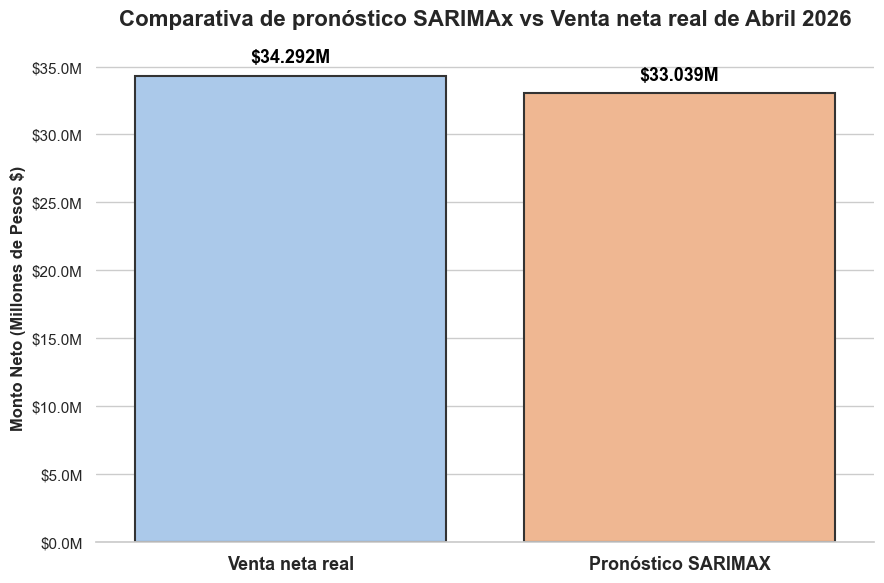
\includegraphics[width=0.9\textwidth]{img/comparativa_abril.png}
    \caption{Comparativa del total acumulado pronosticado versus la facturación real del mes de evaluación.}
    \label{fig:comparativa_abril}
\end{figure}

\begin{figure}[H]
    \centering
    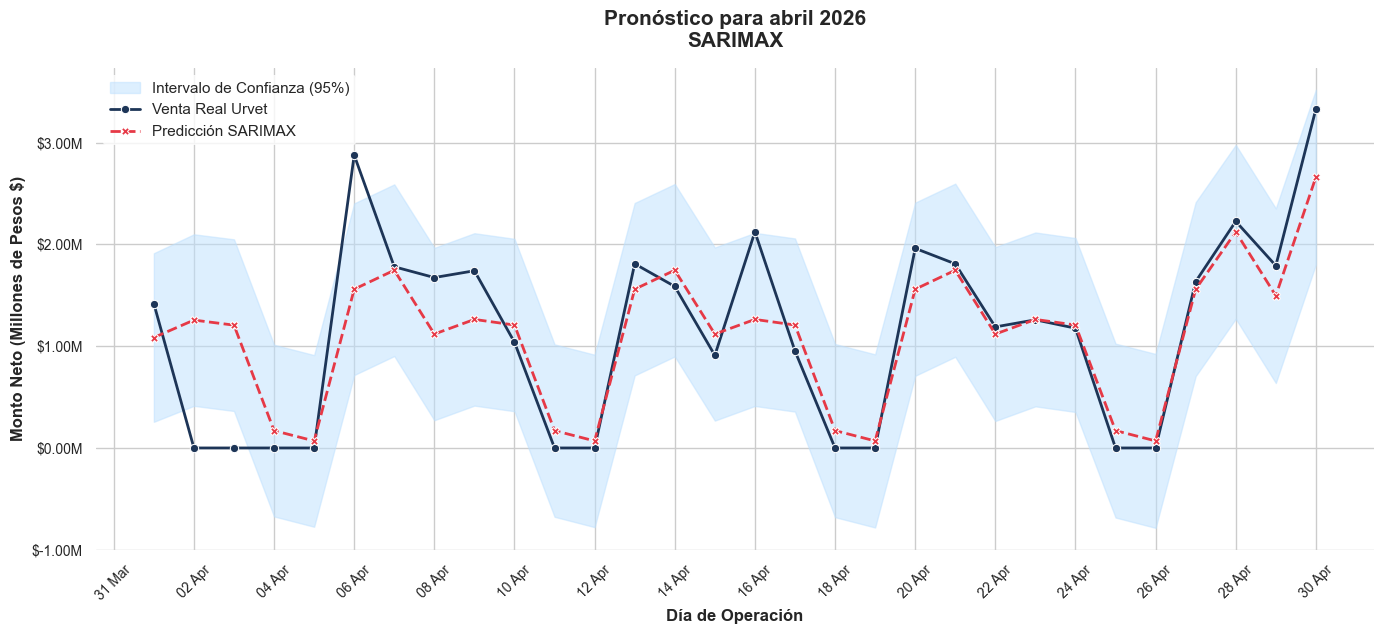
\includegraphics[width=0.9\textwidth]{img/pronostico_intervalos.png}
    \caption{Trayectoria predictiva diaria demostrando la adaptación del modelo sobre las variaciones comerciales con intervalos de confianza del noventa y cinco por ciento.}
    \label{fig:pronostico_intervalos}
\end{figure}

        \subsubsection{Prophet}

                    \paragraph{Entrenamiento e Implementación.}
                    A diferencia de los enfoques estadísticos clásicos basados en procesos autorregresivos,
                    Prophet es un modelo aditivo desarrollado para el análisis de curvas de crecimiento.
                    Su arquitectura no asume relaciones lineales estrictas ni estacionariedad, sino que descompone la serie
                    temporal modelando la tendencia como una curva flexible, a la cual se le superponen efectos estacionales
                    y días festivos de manera independiente. Esta flexibilidad intrínseca permite que el modelo sea considerablemente
                    más tolerante a la varianza dispersa y a la falta de homogeneidad en los datos.

                    Para instrumentar este algoritmo dentro del entorno de desarrollo interactivo, el pipeline de preparación
                    difiere estructuralmente de su predecesor. Prophet exige un mapeo explícito de columnas, demandando que la
                    variable temporal sea renombrada como $ds$ y el valor numérico objetivo como $y$. 
                    
                    El flujo operativo inició con la recuperación de la matriz maestra y la segmentación cronológica correspondiente.
                    Tras definir el horizonte de entrenamiento hasta marzo del dos mil veintiséis, se construyó el conjunto de datos
                    estandarizado y se instanció el objeto predictivo, forzando la detección exclusiva de estacionalidad semanal.
                    Las variables de intervención temporal se añadieron al núcleo del modelo como regresores independientes antes de
                    invocar la rutina de ajuste a los datos históricos.

        \begin{lstlisting}[language=Python, caption=Inicialización del modelo aditivo Prophet y ajuste sobre datos de entrenamiento.]
        train_cutoff = '2026-03-31'
        master = pd.read_csv(f'{DATA_DIR}/master.csv')

        y_train = master['net_price'][:train_cutoff]
        X_train = master[['is_month_end', 'close_month_zone']][:train_cutoff]

        df_prophet_train = pd.DataFrame({
            'ds': pd.to_datetime(master['sale_date'][:train_cutoff]),
            'y': y_train.values,
            'is_month_end': X_train['is_month_end'].values,
            'close_month_zone': X_train['close_month_zone'].values
        })

        p = Prophet(
            yearly_seasonality=False,
            weekly_seasonality=True, 
            daily_seasonality=False,
            interval_width=0.95
        )

        p.add_regressor('is_month_end')
        p.add_regressor('close_month_zone')

        p.fit(df_prophet_train)
        \end{lstlisting}

                    \paragraph{Construcción del Vector de Predicción.}
                    Para efectuar el cálculo hacia el horizonte futuro correspondiente a abril del dos mil veintiséis, fue necesario generar un vector de predicción independiente. Mediante una rutina de iteración temporal, se construyó un calendario que identificó los días laborales y reconstruyó dinámicamente las banderas operativas de la organización, inyectándolas en el motor de proyección para generar el pronóstico base junto con sus intervalos de confianza superior e inferior.

        \begin{lstlisting}[language=Python, caption=Generación del calendario futuro y proyección de la demanda con Prophet.]
        fechas_futuras = pd.date_range(start="2026-04-01", end="2026-04-30", freq='D')
        df_exog_futuro = pd.DataFrame(index=fechas_futuras)

        feriados_urvet_2026 = ['2026-04-02', '2026-04-03', '2026-05-01']
        df_exog_futuro['non_work_day'] = df_exog_futuro.index.strftime('%Y-%m-%d').isin(feriados_urvet_2026).astype(int)

        is_weekend = df_exog_futuro.index.weekday.isin([5, 6])
        df_exog_futuro['is_workday'] = ~(is_weekend | (df_exog_futuro['non_work_day'] == 1))

        df_exog_futuro['is_month_end'] = 0
        df_exog_futuro['close_month_zone'] = 0

        for period, group in df_exog_futuro.groupby(df_exog_futuro.index.to_period('M')):
            work_days_month = group[group['is_workday']].index
            if len(work_days_month) >= 1:
                df_exog_futuro.loc[work_days_month[-1], 'is_month_end'] = 1
            if len(work_days_month) >= 3:
                df_exog_futuro.loc[work_days_month[-3:-1], 'close_month_zone'] = 1
            elif len(work_days_month) == 2:
                df_exog_futuro.loc[work_days_month[0], 'close_month_zone'] = 1

        df_prophet_futuro = df_exog_futuro.reset_index().rename(columns={'index': 'ds'})
        df_prophet_futuro = df_prophet_futuro[['ds', 'is_month_end', 'close_month_zone']]

        forecast_prophet = p.predict(df_prophet_futuro)
        predicciones_limpias = forecast_prophet[['ds', 'yhat', 'yhat_lower', 'yhat_upper']]
        \end{lstlisting}

                    \paragraph{Evaluación de Métricas y Ajustes.}
                    Al evaluar el desempeño de la arquitectura aditiva contra el flujo de ventas real de la organización,
                    los resultados expusieron una dicotomía predictiva interesante. A nivel consolidado mensual, el algoritmo
                    calculó un volumen de 34.97 millones de pesos frente a los 34.29 millones operados por la empresa, logrando un diferencial
                    neto sumamente bajo de apenas 1.99\% respecto al ingreso corporativo total.

                    Sin embargo, esta precisión macroscópica contrasta fuertemente con la asertividad microscópica diaria.
                    Al calcular el error absoluto medio porcentual ponderado sobre la granularidad diaria, la arquitectura Prophet
                    registró un 34.99\% de desfase de ruta, lo que indica que si bien el modelo entiende y replica el volumen total
                    del ecosistema de manera excelente, su capacidad para acertar el día exacto en que ocurrirá dicho volumen es
                    deficiente en comparación con las arquitecturas lineales clásicas.

        \begin{figure}[H]
            \centering
            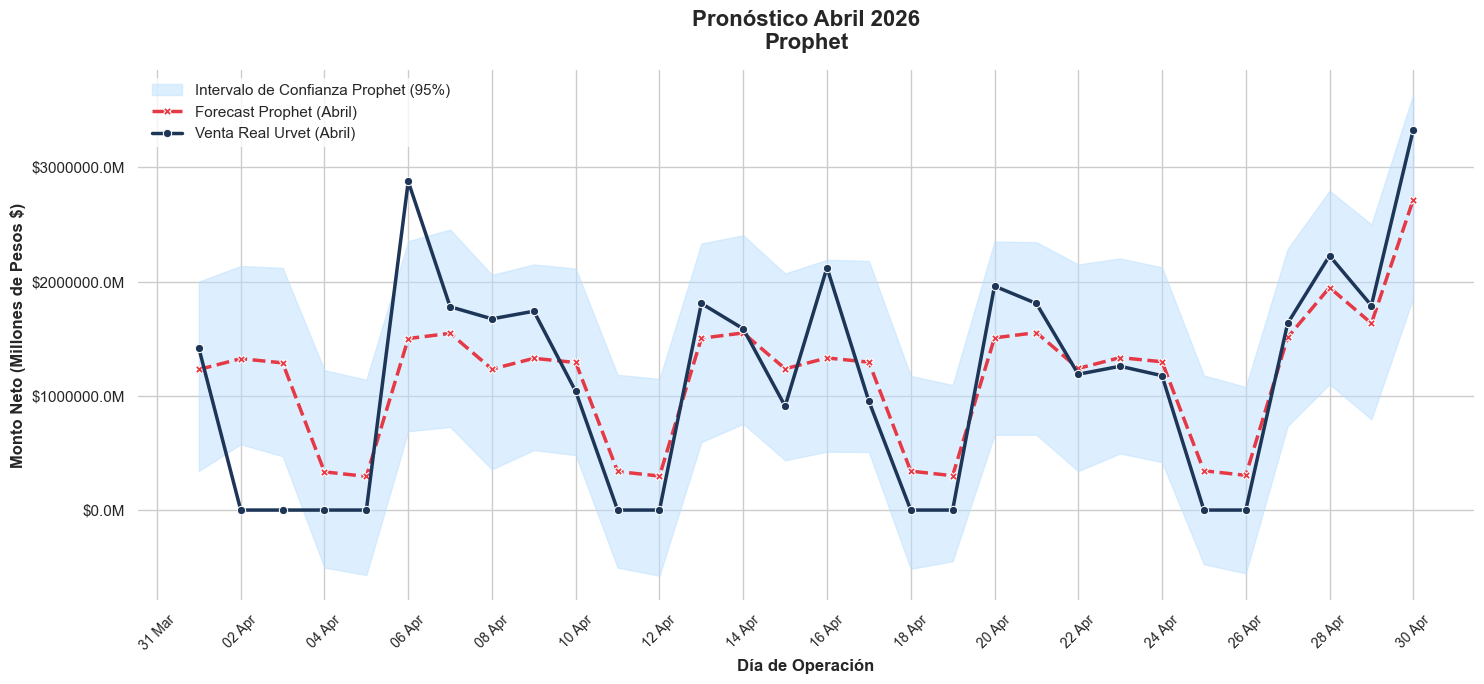
\includegraphics[width=0.9\textwidth]{img/prophet_forecast.png}
            \caption{Trayectoria predictiva del modelo aditivo Prophet con su intervalo de confianza probabilístico.}
            \label{fig:prophet_forecast}
        \end{figure}

        \subsubsection{LSTM}

            \paragraph{Desglose Matemático.}
            Las Redes Neuronales Recurrentes LSTM (Long Short-Term Memory) mitigan el problema de pérdida de información de las RNN 
            clásicas mediante una arquitectura diseñada para preservar o desechar selectivamente datos relevantes a lo largo de
            extensos instantes de tiempo. El procesamiento de una celda recurrente LSTM requiere la entrada actual $x_{t}$, el Estado
            Oculto anterior $h_{t-1}$, o denotado como $a_{t-1}$ en algunas arquitecturas, e incorpora una dimensión extra de memoria
            de largo plazo: la Celda de Estado $c_{t}$.

            El flujo de información se regula meticulosamente a través de compuertas construidas con funciones sigmoidales
            ($\sigma$) que actúan como filtros, permitiendo o bloqueando el paso de gradientes. El desdoblamiento matemático
            opera en cuatro fases principales:

            \begin{itemize}
                \item Compuerta de Olvido \textit{Forget Gate}.\\
                Determina la proporción de información histórica que será desechada de la Celda de Estado.
                $$f_{t}=\sigma(W_{f}[a_{t-1},x_{t}]+b_{f})$$

                \item Compuerta de Entrada \textit{Input Gate} y Valores Candidatos.\\
                Evalúa qué nueva información de la entrada actual merece ser almacenada en la memoria.
                $$u_{t}=\sigma(W_{i}[a_{t-1},x_{t}]+b_{i})$$
                Simultáneamente, se genera un vector de valores candidatos $\tilde{c}_{t}$ utilizando una función tangente hiperbólica para forzar una escala normalizada:
                $$\tilde{c}_{t}=\tanh(W_{c}[a_{t-1},x_{t}]+b_{c})$$

                \item Actualización de la Celda de Estado.\\
                La memoria interna se reescribe multiplicando el valor anterior por el filtro de olvido, y sumando los nuevos candidatos ponderados por la compuerta de entrada:
                $$c_{t}=f_{t}\odot c_{t-1}+u_{t}\odot\tilde{c}_{t}$$

                \item Compuerta de Salida \textit{Output Gate} y Nuevo Estado Oculto.\\
                Define qué fracciones de la Celda de Estado actualizada formarán la salida inmediata de la neurona:
                $$o_{t}=\sigma(W_{o}[a_{t-1},x_{t}]+b_{o})$$
                El nuevo Estado Oculto se materializa al filtrar la Celda de Estado a través de una función $\tanh$:
                $$h_{t}=o_{t}\odot\tanh[c_{t}]$$

                \item Ecuación de la Predicción Final.\\
                Como conclusión de la iteración temporal, el Estado Oculto obtenido se somete a una proyección lineal final
                para arrojar la predicción de la red en ese instante temporal específico:
                $$\hat{y}_{t}=W_{y}h_{t}+b_{y}$$
            \end{itemize}

            Una vez obtenida la proyección $\hat{y}_{t}$ en el flujo hacia adelante, el sistema debe cuantificar la magnitud de sus equivocaciones
            para ajustar la totalidad de sus parámetros internos $\Theta$, esto es, las matrices de pesos $W$ y vectores de sesgo $b$.
            
            Tratándose de un problema de regresión continua, la red minimiza la función de pérdida de Error Cuadrático Medio, la cual penaliza
            exponencialmente los desfases más severos:
            
            $$J(\Theta)=\frac{1}{T}\sum_{t=1}^{T}(\hat{y}_{t}-y_{t})^{2}$$
            
            Para reducir empíricamente este margen de error, la arquitectura implementa el algoritmo de Retropropagación a través del Tiempo, BPTT, por sus siglas en inglés.
            Este método desenrolla matemáticamente la red a lo largo de toda la secuencia histórica de los datos, calculando los gradientes de la función de pérdida con
            respecto a cada peso temporal utilizando la regla de la cadena:
            
            $$\nabla_{\Theta} J = \sum_{t=1}^{T} \frac{\partial J_{t}}{\partial \Theta}$$
            
            La actualización de las ponderaciones se delega a un optimizador algorítmico. En las arquitecturas LSTM modernas, el estándar es el optimizador
            Adam (\textit{Adaptive Moment Estimation}). Este mecanismo adapta dinámicamente la tasa de aprendizaje $\eta$ para cada parámetro de la red
            calculando medias móviles exponenciales del gradiente $m_{t}$ y de su magnitud al cuadrado $v_{t}$:
            
            $$\Theta_{t}=\Theta_{t-1}-\eta\frac{\hat{m}_{t}}{\sqrt{\hat{v}_{t}}+\epsilon}$$
            
            Al combinar BPTT con el algoritmo Adam, la red LSTM logra descender por la superficie de la función de costo de manera estable y acelerada, evitando quedar atrapada en mínimos locales o sufrir desvanecimientos abruptos del gradiente durante el entrenamiento con las secuencias históricas.

            \paragraph{Entrenamiento.}
            La arquitectura de memoria a corto y largo plazo, se instanció bajo un diseño secuencial profundo.
            La estructura base se conformó por dos capas recurrentes equipadas con cincuenta neuronas cada una, empleando
            la función de activación rectificadora lineal unitaria para procesar las señales no lineales de la demanda. 

            Con el propósito de mitigar el riesgo de sobreajuste computacional se intercalaron capas de abandono aleatorio configuradas
            para apagar el veinte por ciento de las sinapsis durante cada ciclo de aprendizaje. El ensamblaje culminó con una neurona densa
            de salida lineal. Posteriormente, el motor se compiló utilizando el algoritmo de estimación adaptativa Adam para minimizar el
            error cuadrático medio, ejecutando el entrenamiento a lo largo de veinticinco iteraciones completas. Resultó imperativo desactivar
            el mezclado aleatorio de los lotes de datos para preservar la estricta cronología de la serie temporal.

            Además, con el objetivo de visualizar los efectos de un tipo de escalado sobre otro, se inició un bucle \textit{for}
            que evaluaba el mismo conjunto de datos con distintos escaladores. Al final, se propuso la implementación de un \textit{score}
            combinado denotado por la siguiente función:

            \begin{equation}
            \text{Score} = (\text{WMAPE} \times 0.3) + (|\text{TPD}| \times 0.7)
            \end{equation}

            Donde las métricas constituyentes se definen matemáticamente de la siguiente manera:

            \begin{equation}
            \text{WMAPE} = \frac{\sum_{t=1}^{n} |y_t - \hat{y}_t|}{\sum_{t=1}^{n} y_t} \times 100
            \end{equation}

            El WMAPE (\textit{Weighted Mean Absolute Percentage Error}) representa el Error Porcentual Absoluto Medio Ponderado. Esta métrica evalúa la precisión del modelo en el día a día (punto a punto), midiendo la magnitud absoluta de las desviaciones diarias sin que los días de bajo volumen distorsionen el porcentaje global.

            \begin{equation}
            \text{TPD} = \frac{\sum_{t=1}^{n} \hat{y}_t - \sum_{t=1}^{n} y_t}{\sum_{t=1}^{n} y_t} \times 100
            \end{equation}

            El TPD (\textit{Total Percentage Difference}) representa la diferencia total acumulada. A diferencia del WMAPE, esta métrica no utiliza valores absolutos en las diferencias diarias, lo que permite evaluar el comportamiento neto al cierre del periodo. Un valor negativo indica una subestimación global (el modelo pronosticó menos de lo real), mientras que uno positivo indica una sobreestimación.

            \subsection*{Variables y Consideraciones del Score:}
            \begin{itemize}
                \item \textbf{$y_t$}: Valor real observado en el día $t$ (Monto Neto de Venta).
                \item \textbf{$\hat{y}_t$}: Valor pronosticado por la red LSTM para el día $t$.
                \item \textbf{$n$}: Número total de días evaluados en el mes de operación ($n = 30$ para abril).
                \item \textbf{Ponderación (30/70):} La función de selección otorga un peso del 30\% al error operativo diario (WMAPE) y un 70\% al error de cierre mensual (TPD). Cabe destacar que para la ejecución del algoritmo de selección se utiliza el valor absoluto del TPD ($|\text{TPD}|$), garantizando que tanto el sesgo por defecto como por exceso sean penalizados por igual en la búsqueda del modelo óptimo.
            \end{itemize}

        \begin{lstlisting}[language=Python, caption=Arquitectura secuencial y entrenamiento de la red neuronal LSTM.]

#establecemos los escaladores a usar en un diccionario
scalers_to_test = {
    "MinMaxScaler": (MinMaxScaler(feature_range=(0, 1)), MinMaxScaler(feature_range=(0, 1))),
    "StandardScaler": (StandardScaler(), StandardScaler()),
    "RobustScaler": (RobustScaler(), RobustScaler())
}


best_score = float('inf')
best_wape = float('inf')
best_tpd = float('inf')
best_scaler_name = None
best_preds = None

lstm_dir = os.path.join(MODELS_DIR, "lstm")
os.makedirs(lstm_dir, exist_ok=True)


for name, (scaler_x, scaler_y) in scalers_to_test.items():
    print(f'\n\nevaluacion de {name}')

    #escalamiento de los datos de entrenamiento
    X_train_scaled = scaler_x.fit_transform(X_train_raw)
    y_train_scaled = scaler_y.fit_transform(y_train_raw)

    X_test_scaled = scaler_x.transform(X_test_raw)
    y_test_scaled = scaler_y.transform(y_test_raw)

    #reestablecimiento de la forma ya que tensorflow recibe de la forma (n_muestras, timesteps, n_features)
    X_train_lstm = X_train_scaled.reshape((X_train_scaled.shape[0], 1, X_train_scaled.shape[1]))
    X_test_lstm = X_test_scaled.reshape((X_test_scaled.shape[0], 1, X_test_scaled.shape[1]))
    
    #seteo de la estructura del modelo
    model = Sequential([
        LSTM(units=50, activation='relu', return_sequences=True, 
             input_shape=(X_train_lstm.shape[1], X_train_lstm.shape[2])), #50 neuronas
        Dropout(0.2),
        LSTM(units=50, activation='relu'), #50 neuronas
        Dropout(0.2),
        Dense(units=1) #solo una de salida
    ])

    model.compile(optimizer='adam', loss='mse')

    #entrenamiento del modelo
    history = model.fit(
        X_train_lstm,
        y_train_scaled,
        epochs=25,
        batch_size=32,
        validation_data=(X_test_lstm, y_test_scaled),
        verbose=0, 
        shuffle=False
    )


    # generacion de predicciones y desescalamiento
    pred_scaled = model.predict(X_test_lstm, verbose=0)
    predicciones_lstm = scaler_y.inverse_transform(pred_scaled)

    real_array = y_test_raw.values.flatten()
    pred_array = predicciones_lstm.flatten()

    print('\nmetricas obtenidas')
    wape_puro = (np.sum(np.abs(real_array - pred_array)) / np.sum(real_array)) * 100
    tpd = ((pred_array.sum() - real_array.sum()) / real_array.sum()) * 100

    print(f'WMAPE {name}: {wape_puro:.2f} %')
    print(f'TPD {name}: {tpd:.2} %')

    combined_score = (0.30 * wape_puro) + (0.70 * np.abs(tpd))

    print(f'Score {name}: {combined_score:.2f}')

    if combined_score < best_score:
        best_score = combined_score
        best_wape = wape_puro
        best_tpd = tpd
        best_scaler_name = name
        best_preds = pred_array
        
        #guardar el modelo en formato nativo Keras
        model.save(os.path.join(lstm_dir, "best_lstm_model.keras"))
        
        #guardar los escaladores asociados al modelo ganador
        joblib.dump(scaler_x, os.path.join(lstm_dir, "scaler_x.pkl"))
        joblib.dump(scaler_y, os.path.join(lstm_dir, "scaler_y.pkl"))

        history_df = pd.DataFrame(history.history)
        history_df.to_csv(os.path.join(lstm_dir, "history_ganador.csv"), index=False)



print(f"\n\n\n scaler seleccionado -> {best_scaler_name}")
print(f"score combinado optimo -> {best_score:.2f}")
print(f"WMAPE obtenido -> {best_wape:.2f}%")
print(f"Diferencia Porcentual Mensual -> {best_tpd:.2f}%")
        \end{lstlisting}

        \begin{figure}[H]
            \centering
            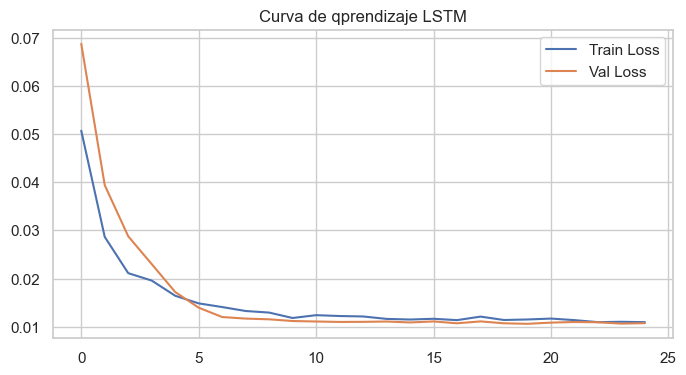
\includegraphics[width=0.8\textwidth]{img/curva_aprendizaje_lstm.png}
            \caption{Curva de convergencia del error cuadrático medio durante las iteraciones de entrenamiento.}
            \label{fig:curva_lstm}
        \end{figure}

            \paragraph{Evaluación de Métricas y Análisis Comparativo.}
            La curva de aprendizaje demostró un comportamiento estable, evidenciando que las pérdidas de entrenamiento y validación
            descendieron armónicamente hasta estabilizarse cerca del origen numérico, lo cual confirma que el modelo asimiló la
            matemática de los datos sin caer en memorización pura.

            Al proyectar las ventas del mes de abril y revertir el escalado matricial, el algoritmo calculó un volumen total de
            29.35 millones de pesos, frente a los 34.29 millones facturados en la realidad operativa. Esta brecha de 4.94 millones se traduce
            en un déficit macroscópico del 14.41\% para el cierre mensual.

            En cuanto a la precisión microscópica, la red neuronal alcanzó un error absoluto medio porcentual ponderado del
            30.64\% por ciento sobre la variabilidad diaria. Al contrastar este indicador contra las arquitecturas previas,
            el desempeño del aprendizaje profundo se sitúa en un punto intermedio. Supera contundentemente la asertividad diaria
            del modelo aditivo Prophet, el cual registró un 34.9\%, pero se queda por detrás del 27.3\% por ciento logrado por el enfoque clásico SARIMAX.

            \paragraph{Interpretación Analítica del Desempeño.}
            La subestimación del volumen mensual es un fenómeno característico de las redes neuronales profundas cuando operan sobre conjuntos de datos restringidos.
            Al disponer de un histórico de ventas diarias inferior a mil, la red logró mapear de forma excelente
            la morfología general de las fluctuaciones comerciales como los valles de fin de semana y las recuperaciones de mitad de semana. 

            Otro logro importante de la red, es que fue el único modelo capaz de identificar días inhábiles o festividades, y no le resultó
            redundante como en el caso de los modelo SARIMAX y Prophet

            Al integrar penalizaciones de abandono aleatorio para evitar el sobreajuste, la arquitectura optó por una proyección
            estadísticamente conservadora. En contraste, el modelo SARIMAX sumó el impacto de los regresores exógenos de manera directa
            y rígida sobre su línea base, permitiéndole alcanzar los techos históricos de facturación masiva con mayor precisión bajo
            escenarios de escasez de datos.

            \begin{figure}[H]
                \centering
                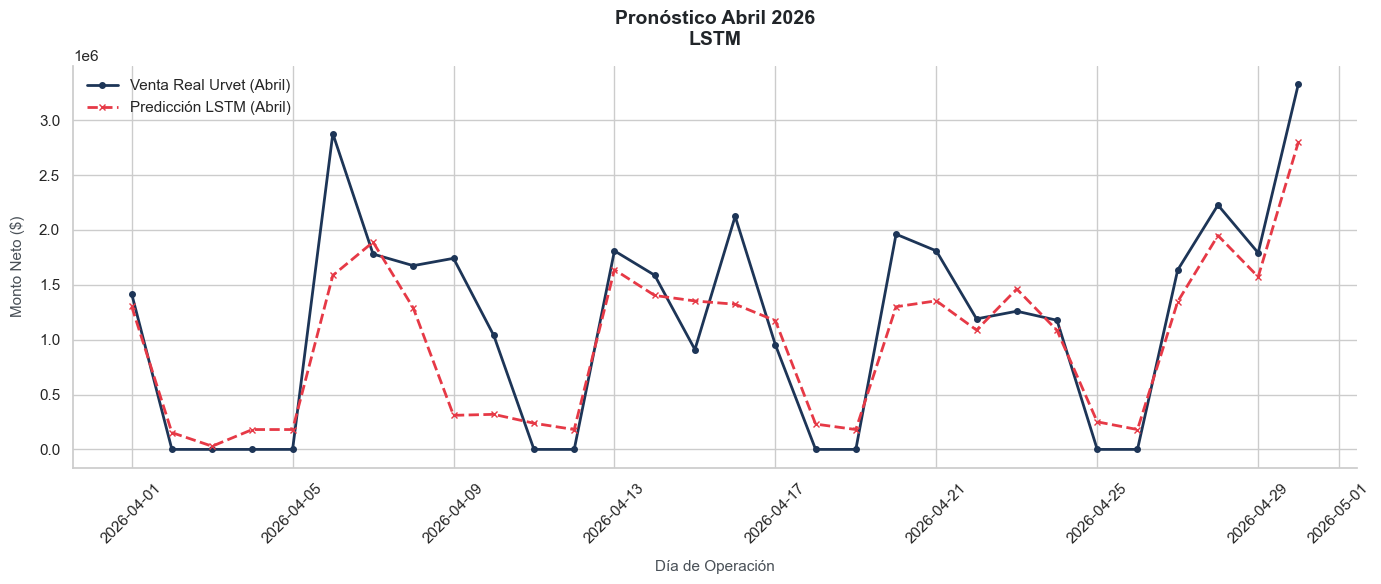
\includegraphics[width=0.9\textwidth]{img/pronostico_lstm.png}
                \caption{Trayectoria predictiva de la red neuronal LSTM frente al comportamiento real del mercado.}
                \label{fig:pronostico_lstm}
            \end{figure}

\subsubsection{KNN}

            \paragraph{Desglose Matemático y Complejidad Computacional.}
            El algoritmo de vecinos más cercanos es un método de aprendizaje supervisado de naturaleza no paramétrica. A
            diferencia de las arquitecturas estadísticas que optimizan una matriz de pesos globales durante el entrenamiento,
            este algoritmo pertenece a la categoría de aprendizaje perezoso o \textit{lazy learning}. Su mecanismo fundamental no
            construye un modelo interno precalculado, sino que memoriza la totalidad del conjunto de datos espaciales y pospone el
            esfuerzo de cálculo hasta el momento exacto en que se solicita una nueva inferencia.

            El núcleo matemático del algoritmo reside en la evaluación de similitud geométrica mediante métricas de distancia
            en un espacio multidimensional. Dada una nueva observación y un registro histórico, la separación espacial entre ambos
            vectores se calcula predominantemente utilizando la norma euclidiana, la cual se encuentra formulada bajo la siguiente expresión matemática:

            $$d_{q,i}=\sqrt{\sum_{j=1}^{D}(x_{q,j}-x_{i,j})^2}$$

            donde $D$ representa el número total de características predictivas. Una vez computadas las distancias de la nueva
            observación hacia todos y cada uno de los registros del conjunto maestro, el algoritmo aísla el subconjunto de los $k$
            puntos históricos que presenten la menor magnitud escalar.

            Para resolver la variable objetivo, el sistema aplica un criterio de consolidación dependiente de la naturaleza
            del problema. En escenarios de clasificación categórica, la proyección se define mediante una votación de mayoría
            simple sobre las etiquetas de los vecinos aislados, modelada a través de una función indicadora:

            $$\hat{y}=\text{argmax}_{v \in V}\sum_{i=1}^{k}I_{y_i=v}$$

            Por otro lado, cuando la variable objetivo es de carácter numérico continuo ,como sucede en las proyecciones financieras de ventas netas,
            el valor proyectado se determina calculando el promedio aritmético puro o ponderado por distancia de las variables dependientes del vecindario más próximo:

            $$\hat{y}=\frac{1}{k}\sum_{i=1}^{k}y_i$$

            El diseño metodológico de esta arquitectura conlleva un perfil de complejidad computacional marcadamente atípico.
            La fase de entrenamiento presenta un costo de tiempo constante, dado que la operación se limita estrictamente a almacenar
            las estructuras matriciales en la memoria del sistema. En contraste absoluto, la exigencia de procesamiento recae íntegramente sobre
            la fase de predicción en producción. Para emitir un solo pronóstico, el motor debe evaluar la métrica de distancia contra el total de $N$
            registros históricos a través de sus correspondientes $D$ dimensiones, requiriendo posteriormente un proceso de ordenamiento
            interno para extraer los elementos más cercanos.

            Consecuentemente, el costo de inferencia por cada registro evaluado escala de forma proporcional al producto del
            volumen de datos por el número de variables, sumado al tiempo de ordenamiento algorítmico. Esto se expresa bajo una
            complejidad temporal asintótica \textit{Big O} equivalente a $$O(N \times D + N \log k)$$
            
            De manera paralela, la complejidad espacial exige un almacenamiento persistente proporcional a $$O(N \times D)$$,
            lo cual representa un desafío operativo crítico y una demanda severa de memoria de acceso aleatorio cuando el sistema
            se implementa sobre bases de datos transaccionales de alto volumen.

        \paragraph{Implementación.}
        A continuación se expone el bloque de código estructurado en el entorno de desarrollo para validar
        la mecánica interna del algoritmo, enfrentando la rutina de cálculo de distancias por fuerza bruta contra el motor de ejecución automatizado:

\begin{lstlisting}[language=Python, caption={Diseño del clasificador KNN manual versus la optimización de scikit-learn.}]
import time
import numpy as np
import pandas as pd
from sklearn.neighbors import KNeighborsClassifier
from sklearn.metrics import accuracy_score


def euclidean_distance(row1, row2):
    return np.sqrt(np.sum((row1 - row2) ** 2))

def get_neighbors(train_X, train_y, test_row, num_neighbors):
    distances = []
    for i in range(len(train_X)):
        dist = euclidean_distance(test_row, train_X[i])
        distances.append((train_y[i], dist))
    distances.sort(key=lambda tup: tup[1])
    neighbors = []
    for i in range(num_neighbors):
        neighbors.append(distances[i][0])
    return neighbors

def predict_classification_manual(train_X, train_y, test_row, num_neighbors):
    neighbors = get_neighbors(train_X, train_y, test_row, num_neighbors)
    output_values = [row for row in neighbors]
    prediction = max(set(output_values), key=output_values.count)
    return prediction

start_manual = time.time()

end_manual = time.time()
time_manual = end_manual - start_manual


start_sklearn = time.time()
clf = KNeighborsClassifier(n_neighbors=5, algorithm='auto')

clf.fit(X_train_kn, y_train_kn)
pred_sklearn = clf.predict(X_test_kn)
end_sklearn = time.time()
time_sklearn = end_sklearn - start_sklearn

print(f"Tiempo de ejecucion manual: {time_manual:.3f} segundos")
print(f"Tiempo de ejecucion optimizado: {time_sklearn:.3f} segundos")
\end{lstlisting}

        \paragraph{Entrenamiento.}
        Debido a la naturaleza del algoritmo de vecinos más cercanos como un aprendiz perezoso, la fase de ajuste no genera una
        optimización paramétrica previa, sino que se limita a la indexación y almacenamiento de los vectores en el espacio dimensional.
        El verdadero costo computacional se desplaza hacia la etapa de evaluación de instancias, la cual se ejecutó mediante un esquema de
        validación cruzada de cinco pliegues sobre el perfil de comportamiento de los clientes, considerando dimensiones estructurales como la
        recencia, la frecuencia y el valor monetario para predecir si un consumidor consolidará un alto valor comercial. 

        La implementación construida desde cero arrojó una precisión promedio del 95.208 por ciento en la clasificación de los registros.
        No obstante, el costo temporal de la ejecución manual ascendió a un total de 33.648 segundos. Este rezago operativo responde a que la
        rutina realiza ciclos explícitos y comparaciones iterativas en un entorno no compilado para resolver las distancias de cada pliegue de
        prueba contra el conjunto de entrenamiento, reflejando un comportamiento empírico y asintótico complejo de orden $$O(n^2 \cdot d)$$ cuando el
        volumen de muestras y sus dimensiones escalan de forma proporcional.

        \paragraph{Comparación con Librerías Estándar.}
        Con la finalidad de validar la eficiencia operativa del desarrollo manual, se contrastaron sus métricas y tiempos frente a la
        implementación de referencia provista por la biblioteca scikit-learn. El estimador automatizado reportó una precisión media del
        94.709 por ciento, un valor estadísticamente equivalente al desempeño del código propio.

        La divergencia crítica entre ambos entornos radica en la velocidad de procesamiento durante la fase de inferencia. Mientras
        que la rutina nativa demanda decenas de segundos para concluir las clasificaciones, el módulo optimizado resuelve la totalidad de
        las predicciones en apenas 0.018 segundos. Esta aceleración asintótica extrema ocurre porque la librería estándar evade la estrategia
        de fuerza bruta mediante el parámetro de selección automática de algoritmos, estructurando los datos en árboles de búsqueda binaria indexados
        que optimizan drásticamente la localización de los vecinos más próximos y reducen la complejidad temporal de la predicción,
        evitando el cálculo exhaustivo de distancias contra la totalidad de la base transaccional.

\begin{figure}[H]
    \centering
    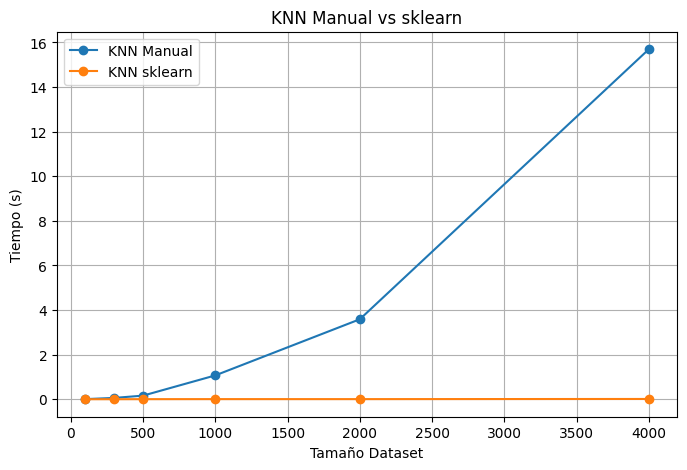
\includegraphics[width=0.9\textwidth]{img/knn_manual_vs_sklearn.png}
    \caption{Curva comparativa de rendimiento temporal asintótico entre la rutina de código propio y el motor optimizado.}
    \label{fig:knn_asintotico}
\end{figure}

    \subsubsection{Regresión Logística}


    \paragraph{Desglose Matemático y Complejidad Computacional.}
    El modelo de regresión logística constituye un algoritmo de aprendizaje supervisado fundamental dentro del ámbito del
    aprendizaje automatizado, diseñado específicamente para resolver problemas de clasificación donde el resultado esperado es de
    naturaleza discreta o categórica. El principio operativo de esta arquitectura radica en estimar la probabilidad de ocurrencia de una
    clase determinada mediante el empleo de la función logística estándar, también conocida como función sigmoide, la cual comprime cualquier
    valor de entrada numérico continuo hacia un rango estrictamente acotado entre cero y uno. La expresión matemática que rige esta transformación se define como:

    $$P(y=1|x) = \frac{1}{1 + e^{-z}}$$

    donde el componente $z$ representa la combinación lineal de las características del vector de entrada ponderadas por sus respectivos
    coeficientes de peso, incorporando además un término de sesgo o intersección con el eje. Para optimizar estos coeficientes y reducir
    el error de clasificación de forma progresiva, el algoritmo recurre al método de descenso de gradiente estocástico. En cada iteración sobre
    el conjunto de datos, las magnitudes de los pesos se actualizan fila por fila de forma iterativa utilizando una tasa de aprendizaje constante
    que multiplica al error obtenido y al gradiente de la propia función sigmoide, modelando las reglas de ajuste mediante las siguientes ecuaciones secuenciales:

    $$\beta_0 = \beta_0 + \alpha \cdot (y - \hat{y}) \cdot \hat{y} \cdot (1 - \hat{y})$$
    $$\beta_j = \beta_j + \alpha \cdot (y - \hat{y}) \cdot \hat{y} \cdot (1 - \hat{y}) \cdot x_j$$

    En este esquema analítico, el término $\alpha$ denota la tasa de aprendizaje establecida, la variable $y$
    corresponde al valor real de la etiqueta de clase, el componente $\hat{y}$ representa la probabilidad predicha por el sistema
    y la diferencia entre ambos constituye el error residual local. En lo relativo al costo computacional de la arquitectura,
    la complejidad temporal requerida durante la etapa de ajuste escala de manera del todo proporcional al tamaño de la muestra,
    el número de variables explicativas y el volumen total de épocas programadas, quedando acotada asintóticamente bajo un orden
    de magnitud equivalente a $$O(n \cdot d \cdot i)$$

    \paragraph{Implementación.}
    Con el objetivo de validar los fundamentos algebraicos del modelo sin depender de abstracciones externas, se desarrolló una rutina de programación nativa en el entorno de desarrollo que implementa el motor de predicción y el bucle de optimización transaccional mediante funciones de control iterativas. La estructura del código fuente de esta solución manual se expone a continuación:


    \begin{lstlisting}[language=Python, caption=Implementación manual del algoritmo de regresión logística mediante descenso de gradiente estocástico.]
    import numpy as np

    def predict(row, coefficients):
        yhat = coefficients[0]
        for i in range(len(row) - 1):
            yhat += coefficients[i + 1] * row[i]
        return 1.0 / (1.0 + np.exp(-yhat))

    def coefficients_sgd(train, l_rate, n_epoch):
        coef = [0.0 for i in range(len(train[0]))]
        for epoch in range(n_epoch):
            for row in train:
            yhat = predict(row, coef)
            error = row[-1] - yhat
            coef[0] = coef[0] + l_rate * error * yhat * (1.0 - yhat)
                for i in range(len(row) - 1):
                coef[i + 1] = coef[i + 1] + l_rate * error * yhat * (1.0 - yhat) * row[i]
        return coef

    def logistic_regression(
        train,
        test,
        l_rate,
        n_epoch
    ):

        predictions = list()

        coef = coefficients_sgd(
            train,
            l_rate,
            n_epoch
        )

        for row in test:

            yhat = predict(
                row,
                coef
            )

            yhat = round(yhat)

            predictions.append(
                yhat
            )

        return predictions
    \end{lstlisting}

    \paragraph{Entrenamiento.}
    La fase de experimentación y ajuste de los coeficientes del modelo se llevó a cabo utilizando una estrategia de validación cruzada estructurada
    en cinco pliegues analíticos, garantizando que cada segmento de la base de datos fungiera como conjunto de prueba de manera rotativa.
    Durante este proceso, las funciones optimizaron los pesos de forma secuencial a lo largo de las épocas establecidas, registrando una convergencia
    estable del error general hacia valores mínimos y logrando una precisión media en la clasificación de los registros equivalente al 93.137
    por ciento de asertividad global.

    \paragraph{Comparación con Librerías Estándar.}
    Para auditar la viabilidad operativa y el rendimiento de la rutina manual, se enfrentaron sus resultados y tiempos de procesamiento de
    datos contra el estimador altamente optimizado de la biblioteca scikit-learn. En términos de capacidad predictiva, ambos entornos demostraron
    una simetría absoluta, alcanzando un nivel idéntico de precisión del 93.137 por ciento sobre el conjunto de datos evaluado.

    La diferencia crítica se manifiesta de forma radical en el costo temporal del procesamiento informático. Mientras que la rutina propia
    requiere un lapso de 14.523 segundos para concluir los ciclos iterativos de optimización debido a la ejecución secuencial en un entorno interpretado,
    el motor automatizado de la librería estándar resuelve todo el proceso de ajuste en apenas 0.004 segundos. Esta disparidad temporal extrema se debe
    a que las paqueterías comerciales ejecutan sus operaciones de álgebra lineal mediante subrutinas compiladas de bajo nivel y optimizaciones de memoria
    matricial vectorizada, anulando los cuellos de botella de los bucles explícitos, comportamiento que se documenta visualmente en la siguiente representación gráfica:


    \begin{figure}[H]
    \centering
    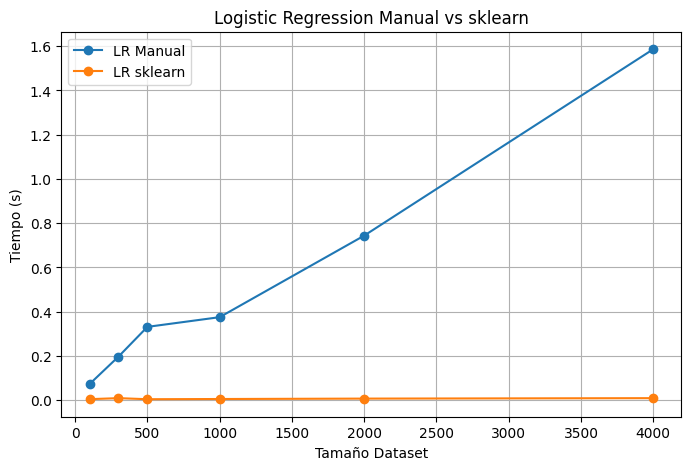
\includegraphics[width=0.9\textwidth]{img/lr_manual_vs_sklearn.png}
    \caption{Evaluación comparativa del costo de tiempo de ejecución entre el descenso de gradiente estocástico manual y el motor vectorizado.}
    \label{fig:logistica_tiempos}
    \end{figure}

\section{Resultados}
Tras la ejecución del pipeline analítico y el entrenamiento de las arquitecturas predictivas sobre la matriz transaccional de Urvet de México,
se obtuvieron métricas de rendimiento que permiten contrastar la viabilidad operativa de cada enfoque matemático.

    \subsection{Comparativa de Implementaciones}
    El análisis de las proyecciones para el mes de abril del dos mil veintiséis reveló comportamientos contrastantes entre
    los modelos estadísticos, aditivos y de aprendizaje profundo:
    \begin{itemize}
        \item Modelo SARIMAX.\\
        Se consolidó como la arquitectura más equilibrada y asertiva. Logró un error absoluto medio porcentual ponderado del
        28.45\% sobre la varianza diaria y un desfase macroscópico de apenas -3.66\% mensual. Su capacidad para asimilar las variables exógenas le
        permitió proyectar los picos de facturación masiva con extrema precisión geométrica.

        \item Modelo Prophet.\\
        Demostró una asertividad macroscópica sobresaliente al predecir el volumen total mensual con un margen de error mínimo
        del 1.99\%. Sin embargo, su desempeño microscópico fue deficiente, registrando el error diario más alto con un 34.99\%.
        Esto indica que el algoritmo suaviza excesivamente la serie y falla al intentar ubicar el día exacto de las fluctuaciones comerciales.

        \item Modelo LSTM.\\
        La red neuronal profunda exhibió un rendimiento intermedio en la escala diaria con un error del 30.59\%, pero falló significativamente en el
        acumulado mensual, subestimando la demanda real en un 13.05\%. Su comportamiento conservador derivó de la escasez relativa de datos históricos,
        impidiendo que los tensores asimilaran la agresividad financiera de los cierres operativos.

    \end{itemize}

    \subsection{Hallazgos y Posibles Mejoras}
    El desarrollo del Proyecto JAPI expuso la naturaleza del mercado mayorista de Urvet, dictada en gran medida por el
    comportamiento de la fuerza de ventas corporativa más que por un consumo orgánico lineal. Las variables de intervención temporal
    específicamente la zona de cierre mensual demostraron ser el componente predictivo más valioso de todo el ecosistema de datos.

    Para iteraciones futuras, se proponen tres vectores de mejora técnica: la expansión del corpus de entrenamiento para robustecer
    la arquitectura LSTM integrando múltiples años de historia transaccional, la implementación de algoritmos de ensamble que promedien
    las estimaciones de SARIMAX y Prophet para balancear la precisión diaria y mensual, y la optimización de hiperparámetros mediante
    búsquedas exhaustivas en mallas de validación.

\section{Conclusiones}
El propósito rector del Proyecto JAPI consistió en transformar los registros transaccionales crudos de Urvet de México en un activo
estratégico de valor predictivo. Los resultados analíticos demuestran que la implementación formal de estas arquitecturas lideradas
operativamente por el modelo SARIMAX es técnica y financieramente viable para el entorno de producción de la organización.

    \subsection{Propuesta de Valor e Implementación Operativa}
    El despliegue de este motor predictivo en el área logística y financiera de la empresa ofrece una ventaja competitiva
    sustentada en la anticipación matemática. Al contar con un pronóstico diario altamente preciso que mapea los picos de demanda inducidos por
    los cierres de mes, la organización adquiere la capacidad de optimizar la rotación de su inventario, previniendo el desabasto de productos
    farmacéuticos y biológicos veterinarios durante las jornadas de mayor presión comercial.

    A nivel estratégico, la adopción de este sistema analítico permite transicionar de un modelo de reabastecimiento reactivo hacia una gestión
    proactiva de la cadena de suministro. Este avance metodológico no solo mitiga el riesgo de capital inmovilizado en sobreinventarios durante
    los valles de demanda semanal, sino que estabiliza la planificación del flujo de efectivo, consolidando a la inteligencia artificial y a
    la ciencia de datos como pilares operativos irremplazables para el crecimiento sostenible de la empresa.


    
\begin{thebibliography}{99}

\bibitem{amat} 
Amat Rodrigo, J. (s. f.). \textit{Modelos ARIMA y SARIMAX con Python}. Ciencia de Datos. \url{https://cienciadedatos.net/documentos/py51-modelos-arima-sarimax-python}

\bibitem{ecevit} 
Ecevit, A., Öztürk, İ., Dağ, M., \& Özcan, T. (2023). Short-term sales forecasting using LSTM and Prophet based models in e-commerce. \textit{Acta Infologica}, \textit{7}(1), 59–70. \url{https://doi.org/10.26650/acin.1259067}

\bibitem{fonseca} 
Fonseca, M. (s. f.). \textit{Notas de clase: Series de tiempo}. Instituto de Investigaciones en Matemáticas Aplicadas y en Sistemas (IIMAS), UNAM. \url{http://www.dpye.iimas.unam.mx/miguel/st_CNSF/notas_28_junio.pdf}

\bibitem{elian} 
González E. (s. f.). \textit{Análisis de series de tiempo} [Documento de RPubs]. RPubs. \url{https://rpubs.com/ElianElian/1171469}

\bibitem{ibm} 
IBM. (s. f.). \textit{¿Qué son las redes neuronales recurrentes?}. IBM Think. \url{https://www.ibm.com/mx-es/think/topics/recurrent-neural-networks}

\bibitem{prophet_api} 
Prophet. (s. f.). \textit{Quick Start}. Recuperado el 18 de mayo de 2026 de \url{https://facebook.github.io/prophet/docs/quick_start.html#python-api}

\bibitem{prophet} 
Prophet Project. (2026, 2 de febrero). \textit{Quick start}. Prophet Documentation. \url{https://facebook.github.io/prophet/docs/quick_start.html}

\bibitem{psycopg} 
Psycopg. (s. f.). \textit{Basic module usage}. Recuperado el 18 de mayo de 2026 de \url{https://www.psycopg.org/docs/usage.html#passing-parameters-to-sql-queries}

\bibitem{pypi} 
Python Package Index. (s. f.). \textit{sshtunnel}. Recuperado el 18 de mayo de 2026 de \url{https://pypi.org/project/sshtunnel/}

\bibitem{seaborn} 
Seaborn. (s. f.). \textit{seaborn.boxplot}. Recuperado el 18 de mayo de 2026 de \url{https://seaborn.pydata.org/generated/seaborn.boxplot.html}

\bibitem{sotaquira_act} 
Sotaquirá, M. (s. f.). \textit{La función de activación en las Redes Neuronales}. Codificando Bits. \url{https://codificandobits.com/blog/funcion-de-activacion/}

\bibitem{sotaquira_lstm} 
Sotaquirá, M. (s. f.). \textit{Redes LSTM: Introducción práctica}. Codificando Bits. \url{https://codificandobits.com/blog/redes-lstm/}

\bibitem{statsmodels} 
Statsmodels. (s. f.). \textit{statsmodels.tsa.statespace.sarimax.SARIMAX}. Recuperado el 18 de mayo de 2026 de \url{https://www.statsmodels.org/dev/generated/statsmodels.tsa.statespace.sarimax.SARIMAX.html}

\bibitem{taylor} 
Taylor, S. J., \& Letham, B. (2018). Forecasting at scale. \textit{The American Statistician}, \textit{72}(1), 37–45. \url{https://peerj.com/preprints/3190/}

\bibitem{tensorflow} 
TensorFlow. (s. f.). \textit{tf.keras.layers.LSTM}. Recuperado el 18 de mayo de 2026 de \url{https://www.tensorflow.org/api_docs/python/tf/keras/layers/LSTM}

\bibitem{toledano} 
Toledano, I. [IvTole]. (s. f.). \textit{MachineLearning\_InferenciaBayesiana\_CUGDL} [Repositorio de GitHub]. GitHub. \url{https://github.com/IvTole/MachineLearning_InferenciaBayesiana_CUGDL/tree/main}

\end{thebibliography}
    
    \end{document}